\documentclass[paper=a4]{ctexart} % A4 paper and 11pt font size
\usepackage{fontspec,caption, xeCJK,amsmath,tocvsec2,extarrows, chngpage, adjustbox, clrscode}
\usepackage{listings}
\usepackage[T1]{fontenc} % Use 8-bit encoding that has 256 glyphs
\usepackage[english]{babel} % English language/hyphenation
\usepackage{amsmath,amsfonts,amsthm,amssymb, enumerate} % Math packages
\usepackage{framed,floatflt}   
\usepackage{graphics}
\usepackage{graphicx}
\usepackage{picins}
\usepackage{lipsum} % Used for inserting dummy 'Lorem ipsum' text into the template

\usepackage{sectsty} % Allows customizing section commands
% \allsectionsfont{\centering \normalfont\scshape} % Make all sections centered, the default font and small caps
\usepackage{wrapfig}
\usepackage{fancyhdr} % Custom headers and footers
\pagestyle{fancyplain} % Makes all pages in the document conform to the custom headers and footers
\fancyhead{} % No page header - if you want one, create it in the same way as the footers below
\fancyfoot[L]{} % Empty left footer
\fancyfoot[C]{} % Empty center footer
\fancyfoot[R]{\thepage} % Page numbering for right footer
\renewcommand{\headrulewidth}{0pt} % Remove header underlines
\renewcommand{\footrulewidth}{0pt} % Remove footer underlines
\setlength{\headheight}{13.6pt} % Customize the height of the header

\numberwithin{equation}{section} % Number equations within sections (i.e. 1.1, 1.2, 2.1, 2.2 instead of 1, 2, 3, 4)
\numberwithin{figure}{section} % Number figures within sections (i.e. 1.1, 1.2, 2.1, 2.2 instead of 1, 2, 3, 4)
\numberwithin{table}{section} % Number tables within sections (i.e. 1.1, 1.2, 2.1, 2.2 instead of 1, 2, 3, 4)

\lstset{
        keywordstyle=\color{blue}, %设置关键字颜色
        commentstyle=\color[cmyk]{1,0,1,0}, %设置注释颜色
        frame=single, %设置边框格式
        escapeinside=``, %逃逸字符(1左面的键),用于显示中文
        breaklines, %自动折行
        extendedchars=false, %解决代码跨页时,章节标题,页眉等汉字不显示的问题
        xleftmargin=2em,xrightmargin=2em, aboveskip=1em, %设置边距
        tabsize=4, %设置tab空格数
        showspaces=false %不显示空格
       }

\setlength\parindent{0pt} % Removes all indentation from paragraphs - comment this line for an assignment with lots of text

\setcounter{footnote}{-1} %第一个footnote不显示标号

% ----------------------------------------------------------------------------------------
% TITLE SECTION
% ----------------------------------------------------------------------------------------
\newcommand{\horrule}[1]{\rule{\linewidth}{#1}} % Create horizontal rule command with 1 argument of height
\title{
  \normalfont \normalsize 
  \textsc{\\~\\~\\~\\~\\~\\University of Science and Technology of China} \\ [25pt] % Your university, school and/or department name(s)
  \horrule{0.5pt} \\[0.4cm] % Thin top horizontal rule
  \huge 基于Inferno的集群与并行计算框架 \\ % The assignment title
  \horrule{2pt} \\[0.5cm] % Thick bottom horizontal rule
}

\newcommand{\n}{\\\indent}
\author{\Large{阮震元~~~~解宇飞~~~~杨智~~~~刘旭彤}\footnote{阮震元~:~PB13011009,联系方式rzyrzyrzy2014@gmail.com,科技实验楼1406系统设计室}
\setcounter{footnote}{-1}
\footnote{解宇飞~:~PB13011001~~~~杨智~:~PB13011079~~~~刘旭彤~:~PB13011072}
} % Your name
\date{} % Today's date or a custom date

\usepackage{enumitem}

\lstset{
        language=text,
        keywordstyle=\color{blue}, %设置关键字颜色
        commentstyle=\color[cmyk]{1,0,1,0}, %设置注释颜色
        frame=single, %设置边框格式
        escapeinside=``, %逃逸字符(1左面的键),用于显示中文
        breaklines, %自动折行
        extendedchars=false, %解决代码跨页时,章节标题,页眉等汉字不显示的问题
        xleftmargin=2em,xrightmargin=2em, aboveskip=1em, %设置边距
        tabsize=4, %设置tab空格数
        showspaces=false %不显示空格
       }

\newcounter{newlist} %自定义新计数器
\newenvironment{denselist}[1][可改变的列表题目]{%%%%%定义新环境
\begin{list}{\textbf{\hei #1} \arabic{newlist}:} %%标签格式
{
\usecounter{newlist}
\setlength{\labelwidth}{22pt} %标签盒子宽度
\setlength{\labelsep}{0cm} %标签与列表文本距离
\setlength{\leftmargin}{0cm} %左右边界
\setlength{\rightmargin}{0cm}
\setlength{\parsep}{0ex} %段落间距
\setlength{\itemsep}{0ex} %标签间距
\setlength{\itemindent}{44pt} %标签缩进量
\setlength{\listparindent}{22pt} %段落缩进量
}}
{\end{list}}%%%%%      


\begin{document}

\maketitle % Print the title
 
% 目录
% 可以直接编辑toc文件来更改目录
\clearpage
\setcounter{section}{0}
\setcounter{subsection}{0}
\setcounter{subsubsection}{0}
\tableofcontents
\clearpage
% 改变层次目录来达到section和subsection默认不编号(需要tocvsec2包)

\section{调研报告}

\subsection{项目背景及实践意义}

\subsubsection{项目的背景}
如今人类各个学科繁多、涉及面广、分类细致,而且不同学科之间又有交叉.而如今很多的学科都需要进行大量的计算,如天文学研究组织需要计算机来分析太空脉冲,星位移动;生物学家需要计算机来模拟蛋白质的折叠过程;药物学家需要计算机来研制克服爱滋病或非典的药物;数学家需要计算机来计算最大的质数和圆周率的更精确值;经济学家也要用计算机分析计算在几万种因素考虑下某个企业/城市/国家的发展方向从而宏观调控.由此可见,未来科学的发展离不开计算.在很多时候,为了进行研究而特地去购买一台专用的超级计算机往往是不现实的.而分布式计算,因为其高效而便宜的特点,越来越受社会的关注.\n
为了说明目前国内分布式计算的现状,我们参考了BOINC平台的一些数据. \n
BOINC,也即伯克利开放式网络计算平台(Berkeley Open Infrastructure for Network Computing),是目前主流的分布式计算平台之一.作为一个高性能的分布式计算平台,截止至2015年1月16日,BOINC在全球有235,980位活跃的参与者以及692,208台活跃的主机,提供约9.871 petaFLOPS的运算能力(天河二号超级计算机运算速度约为33.86 petaFLOPS).\n
以生命科学为例,下面是一些运行在BOINC平台下的项目:
\begin{enumerate}
\item Discovering Dengue Drugs : 针对登革热、丙型肝炎、西尼罗河病毒和黄热病病毒发现有前途的药物先导化合物
\item Genome Comparison : 染色体对比研究
\item Help Conquer Cancer : 帮助科学家征服癌症
\item Help Defeat Cancer : 帮助科学家对抗癌症
\item Human Proteome Folding : 人类蛋白质折叠研究 
\item Human Proteome Folding 2 : 人类蛋白质折叠第2阶段研究
\item Help Cure Muscular Dystrophy : 针对肌肉营养失调和其他神经肌肉型疾病的研究
\item Nutritious Rice for the World : 针对水稻预测蛋白质结构的研究,以提高水稻产量
\end{enumerate}

\subsubsection{分布式操作系统}
分布式操作系统(Distributed operating system)是在互不依赖的、联网的、相互通信的、物理上分离的多个节点上的软件.每个独立的节点包含一部分整体的操作系统上软件的子集.每个子集都可分为两个不同的部分.第一部分是一个通用的微内核,这个内核直接控制节点上的硬件资源.第二部分是一些高层次的系统管理程序,用来协调节点上独立的和相互协作的活动.这两个部分可以把多节点上的资源和处理能力整合成一个高效并且稳定的系统.因此,尽管这个系统上包含了很多的节点,但是在用户和应用程序看来,这就像是一个节点一样.

\begin{figure}[htbp]
\centering
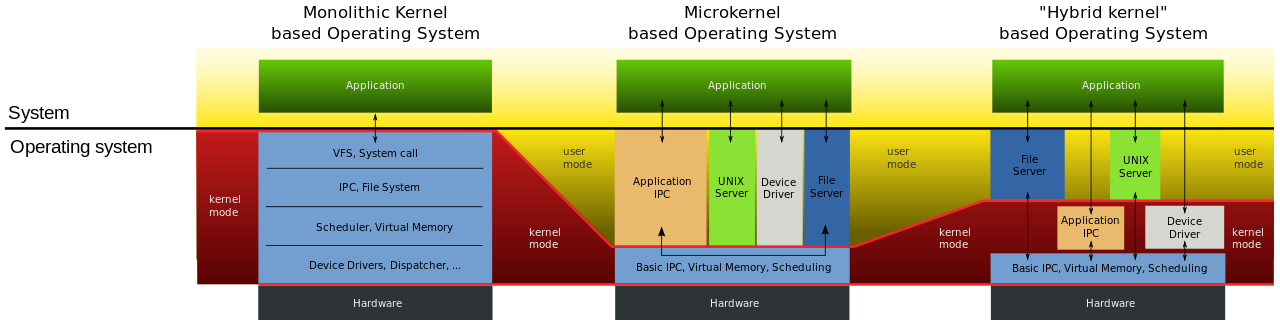
\includegraphics[width=4.8in,height=1.5in]{pic/distribute_os.png}
\caption{分布式操作系统的架构}
\end{figure}


\subsubsection{分布式计算}
分布式计算是指把一个需要拥有强大计算能力的超级计算机才能解决的问题分割成小部分,通过分配给许多计算机单独进行计算,整合汇总的局部结果最终得到最终结果,达到虚拟计算机解决大型问题的效果.\n
如今很多领域都采用了这种用分布式系统搭建集群并实现并行计算的方式来进行复杂问题的处理.例如蛋白质疾病分布式计算项目.这个项目主要研究蛋白质折叠、误折、聚合及由此过程引起的一些相关疾病的分布式计算工程.该项目使用联网式的计算方式和大量的分布式计算能力来模拟蛋白质折叠的过程,该过程需要尽量大量、复杂的计算.通过利用世界各地闲散的计算资源,我们可以加快该项目的进程.

\subsubsection{分布式系统实现并行计算的主要问题}

\begin{enumerate}
\item 分布式的数据和文件管理 : 在搭建起大规模的集群时,必须考虑数据分布存储的管理以及访问问题.唯有解决了这个问题,才能够保证并行计算结果的正确性以及并行计算的性能.
\item 数据访问和通信控制 : 在分布式存储访问结构的系统中,数据在不同节点间传输,由于不同节点的运算速度不一致,此外,还有数据访问/通信的时间延迟等问题的存在,所以必须考虑数据和计算同步问题.
\item 可靠性 : 在某些情况下,如网络连接失败,节点可能会失效,进而导致数据丢失、程序终止、乃至系统崩溃等问题的发生.因此,为保证可靠性,必须考虑数据丢失后的恢复以及程序和系统崩溃后的恢复.
\item 网络互联结构的选择 : 不同的节点链接的结构会对系统整体的可靠性以及整体的运算速度产生重大影响.因此,必须根据实际需要、实际情况,权衡各个因素,选择最合适的节点链接结构,如主从非对称结构、环形结构、互联网络结构等.
\item 并行计算的任务划分和算法设计 : 并行计算需要将一个大的计算任务分解成数量合适的小任务,把这些小任务分配给不同的节点或者处理器进行处理,最终收集各个节点/处理器返回的局部结果,并最终整合为一个大的结果.其中并行计算的形式主要有算法分解和数据划分.在分解和划分时,要充分利用各节点、处理器的性能,从而提高运算速度.
\item 并行计算程序设计框架的设计以及实现 : 为了保证并行计算的正确性以及高效性,程序员需要考虑各种各样繁琐的技术细节:数据的存储管理、计算任务的划分、任务的调度执行、数据和计算的同步、结果的收集、节点实效后的恢复等.如何使这些底层细节透明化、自动实现并行计算,是一个很重要的问题.
\item 如何度量并行计算的性能 : 度量并行计算性能的指标是并行计算技术的核心.
唯有有了一个确定的指标,才能设计出合适的算法以及实现方式.
\end{enumerate}

\subsubsection{Inferno操作系统}

根据调研,我们最终决定使用开源的分布式操作系统Inferno来实现分布式计算.\n
Inferno是一个由贝尔实验室研究发明的开源的分布式操作系统,现在由Vita Nuova继续发展和维护.它基于贝尔实验室plan9的经验和该实验室对os、语言、实时编译器、网络、移植等相关方面的研究.\n
\begin{figure}[htbp]
\centering
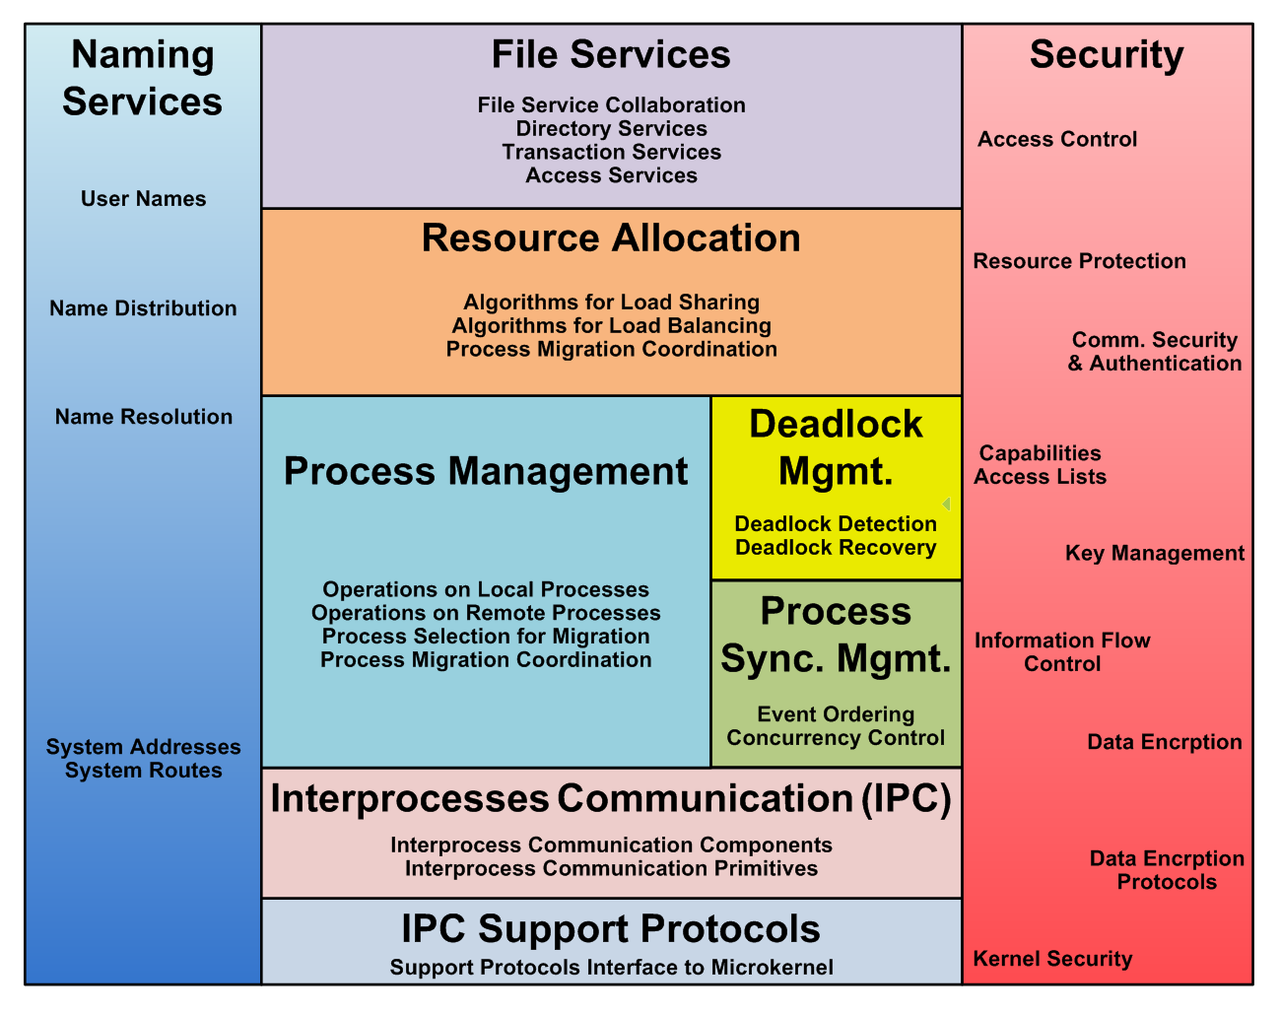
\includegraphics[width=4.8in,height=3.5in]{pic/inferno.png}
\caption{Inferno的架构}
\end{figure}
该系统定义了一个名为Dis的虚拟机,Dis可在不同的机器上实现.\n
Inferno也提供了一个虚拟的、提供相同借口的操作系统,这个操作系统可以让用户在硬件上直接运行Inferno或者在其它系统中以应用程序的方式运行Inferno. \n
为了让应用程序以统一的方式进行文件操作,如打开、关闭、读写,Inferno采用了一种名为Styx的通信协议.\n
作为一个分布式操作系统,Inferno的设计基于以下三个基本原则:
\begin{itemize}
\item Resources as files: 所有的资源都以分层次的文件的形式存在于文件系统中.
\item Namespaces: 在应用程序看来,网络是一个单一的、条理清楚的namespace(命名空间).虽然这个namespace看起来像是一个分层次的文件系统,但实际上,它表示的是分散的资源.
\item Standard communication: 通过一个名为Styx的协议来访问所有本地和远程的资源.
\end{itemize}

\subsection{小组成员相关背景}
\begin{center}
  \bf{阮震元}
\end{center}
\begin{enumerate}
\item 第二届全国RDMA编程挑战赛冠军
\item 现任科大超算曙光队主力队员,7月将代表科大出征国际超算竞赛
\item 高中时获全国信息学联赛一等奖
\item Topcoder SRM DIV 1
\item Coderforces DIV 1
\item 中国最大计算器论坛cnCalc超级版主
 \end{enumerate}
\hspace{0.75cm}
5年编程开发经验,熟悉C,C++,Java,Python,Scala,Pascal,Deiphi等语言,CUDA,OPENMP,MPI等并行技术.有JavaSE,JavaWeb开发经历,Linux运维经验.高中时获信息学联赛一等奖,Topcoder SRM DIV 1,Coderforces DIV 1,有丰富的算法竞赛经历.大二参加全国RDMA编程挑战赛,具体内容是把分布式处理框架Spark\footnote{http://spark.apache.org/}的IO部分从TCP/IP协议移植到RDMA协议,大幅度提高IO吞吐率从而达到加速效果,获冠军.现任科大超算队队员,即将出征今年7月在德国汉堡举行的国际大学生超算竞赛,在队内负责大型分子动力学模拟软件LAMMPS\footnote{http://lammps.sandia.gov/}的优化加速工作.同时在队内担任系统管理员一职,现管理两个超算系统共十余个节点.

\subsection{立项依据}

\subsubsection{项目意义}
本项目的目标是在具有强大可移植性的分布式操作系统Inferno上实现一个通用并行计算框架,使用户在不了解Inferno分布式资源细节的情况下方便地开发并行程序.\n
 目前流行的并行计算框架如:基于消息传递的“裸”并行编程模型MPI:使用Nvdia加速卡的CUDA; 基于同步数据流的MapReduce,Spark,Prlter:基于数据流水线的Dryad/DryadLINQ,SCOPE,基于存储共享的Piccolo,用于图计算的Pregel,Apache等.本项目所实现的基于分布式操作系统Inferno的分布式结构和rstyx网络协议的并行计算框架属于独创性工作.\n
本项目利用Inferno系统方便的分布式资源管理解决了分布式数据存储管理的问题,通过rstys协议解决通信控制问题.\n
相比CUDA而言,我们并不需要特殊的硬件,只需每台节点上装有Inferno.对于OpenMP而言,我们不仅可以和他一样方便使用一条预处理指令即可自动对for,while等实现并行化,还可以直接看到由我们的解释器翻译出来的并行化代码(保证可读性和可扩展性),甚至可以自己再进一步修改优化.相比MPI我们则不需要实现复杂的通信接口,一切都基于Inferno强大的网络协议Styx,Rstyx.相比MapReduce,Spark而言,我们利用Inferno天然的分布式特点,使用脚本即可实现类似于Map,Reduce的函数.

\subsubsection{理论依据}

\paragraph{资源即文件}

所有Inferno的本地和远程资源都被表示为分层文件系统内的一组动态的文件,这些文件可以表示存储设备、进程、服务、网络和网络连接.应用程序可以通过使用标准的文件操作要求来操作相关的文件进而访问每个资源.使用文件为系统中心概念的优点是:
\begin{itemize}
\item 文件系统具有跨多种操作系统的简单和易于理解的界面,文件界面一般有一套定义好的操作,例如打开,读,写.
\item 通过文件系统降低了代码量,并保持Inferno系统简单、可靠和高度轻便的特性.
\item 对众所周知的文件使用惯例命名,便于统一和理解.
\item 便于确定文件的访问权限和文件许可,可以用于确保多级别的安全性.
\end{itemize}
\hspace{0.75cm}文件名和这些文件的动态的内容可以基于每个需求和每个客户端的基础上产生.例如对于一个传感器资源的数据文件在不同的时间读取就会返回不同的输出,或者每次读取都会在新的一行添加一个数据.这种特性是实现并行计算数据共享的基础之一.

\paragraph{命名空间}
 Inferno的第二个关键原理就是可计算的命名空间,通过命名空间每个应用程序会对它需要访问的资源建立一个独一无二的私有视角,所有的资源被表示为文件的层次结构,并且通过标准文件访问操作来访问,一个进程所使用的各种文件和服务都被一个单根分层文件系统组合起来,叫做命名空间.一个名称空间内访问的资源可以位于单个客户端或在整个网络中的多个服务器.\n
    命名空间系统的主要优点是应用程序可以使用的资源完全透明,在应用程序可见的命名空间中挂载的所有动态资源文件,无论是本地的还是远程的,该应用程序都可以方便的访问.例如,一个图形化的调试器通过读取在/prog目录下的动态文件来访问关于目前系统进程的信息,如果用户希望在另一台远程机器上调试,只需将原来那台机器的/prog目录挂入目前这台机器,对于调试器而言,它只是读取在/prog目录中的文件,但并不知道他们来自哪里.

\paragraph{使用标准通信协议来访问资源}
  Inferno使用一个被Inferno内核或应用程序执行的协议来表示或访问资源.因为所有的资源都被表示为文件,包括网络和网络连接,所以需要一个协议来和提供本地与远程资源的通信.这个协议是一个叫9P的文件服务协议(Styx是一个更早的变体).这种方法就为我们利用已知的技术建立添加远程文件系统的分布式系统提供了一个自然的途径.拥有一个标准通信协议还提供了一个关注安全的点,Inferno提供了下面几种安全通信机制:
  \begin{itemize}
  \item 基于证书的用户认证.
  \item 消息加密.
  \end{itemize}

\subsection{目前所调研到的相关工作}

\subsubsection{Inferno相关调研}
对于Inferno系统的调研的目的是利用Inferno系统方便的分布式资源管理以及sytx通信协议来处理集群搭建以及并行框架问题.从目前的网络资源来看,Inferno研发的相关工作主要集中于Inferno的开发团队.\n
我们小组对于Inferno的理解主要来源于Inferno系统自带的documentation(doc目录)以及Inferno官方documentation和tutorial\footnote{http://www.vitanuova.com/Inferno/docs.html}.Bell实验室公开的Documentation\footnote{http://doc.cat-v.org/Inferno/4th\_edition}.\n
Inferno提供了两种模式native和hosted.其中hosted模式是一种应用层虚拟化,可以让Inferno运行在Linux,Win,OSX等系统中.\n
经过我们的调研,Inferno系统的内核有80余万行代码,并且无法取得到其开发日志.另外,Inferno系统已于2010年停止维护.所以我们决定只以Inferno作为分布式资源管理的工具,通过Inferno的shell脚本语言作为开发语言来构建集群并处理并行框架问题.具体的Inferno shell的用法我们参照Roger Peppé的《The Inferno Shell》\footnote{\text{www.vitanuova.com/Inferno/papers/sh.html}}一文进行运用.值得一提的是Inferno的shell非常强大,它核心功能精悍且可以动态加载第三方模块,这一点和python非常相似.\n
关于Inferno的sytx通信协议方面,我们调研到Rob Pike的关于《The Styx Architecture for Distributed Systems》\footnote{www.vitanuova.com/Inferno/papers/styx.html}的工作,了解infeno通过“资源即文件”的思想,将存储设备、进程、服务、网络通信等表示为文件,并通过文件的读、写、执行来控制各种资源或者进行交互.而sytx则是作为简单而统一的网络通信协议,构成了在系统内通信、操作资源架构的核心. 

\subsubsection{常见并行框架概况}
由于我们小组的主要任务还是对并行框架的构建,所以对于各个平台、模型、系统下的分布式计算和并行框架的调研是必不可少的.通过对文献及网络资源的查找,我们小组发现还没有在Inferno系统上构造并行框架的相关研究,所以创新性抑或是独创性是有所保证的.\n
接下来我们小组对几个比较常用的并行框架进行了一定的调研:
\begin{enumerate}
\item MPI : Message Passing Interface (MPI)是一个语言独立的对并行计算机进行编程的通信协议或通信系统.MPI支持点对点或者集群通信,具有标准化和可移植性的特点.''MPI is a message-passing application programmer interface, together with protocol and semantic specifications for how its features must behave in any implementation''\footnote{Gropp, William; Lusk, Ewing; Skjellum, Anthony (1996). ''A High-Performance, Portable Implementation of the MPI Message Passing Interface''. Parallel Computing. CiteSeerX: 10.1.1.102.9485}.在传输层MPI利用了sockets和TCP.MPI模型也因其高性能、可移植性、可扩展性而广泛应用于高性能计算中.
\item OpenMP : Open Multi-Processing是一种支持多平台进行shared memory multiprocessing programming的应用程序接口.OpenMP的核心元素包括进程创建、负载分配、数据环境管理、进程同步等.除了其优秀的跨平台能力外,在集群中OpenMP还可与MPI模型进行混合处理问题.

\begin{figure}[htbp]
\centering
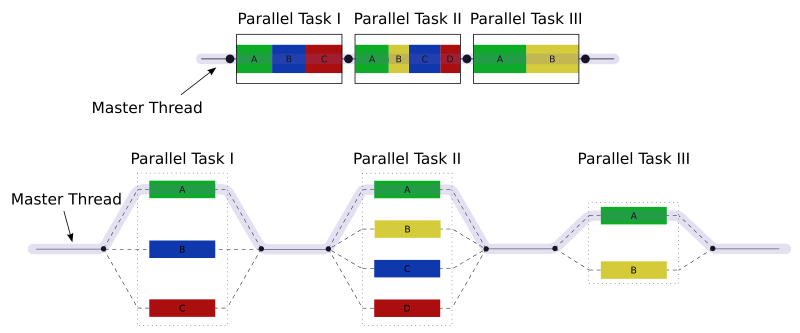
\includegraphics[width=4.8in,height=2in]{pic/openmp.png}
\caption{OpenMP原理}
\end{figure}

\item CUDA : Compute Unified Device Architecture(CUDA)是由英伟达公司创造的,用于GPU上的平行处理平台.利用CUDA,GPU不仅可以进行图形处理,还可进行其他的通用计算(所谓的GPGPU).

对于操作系统,它支持windows、linux、mac os三大主流系统.CUDA为开发者提供了虚拟指令集和并行计算单元的内存来进行运算.

\item TBB(Intel Threading Building Blocks):是一个由英特尔公司开发的C++模板库,主要目的是使得软件开发者更好的利用多核处理器.该库为开发者提供了一些线程安全的容器和算法,使得开发者无需过多关注系统线程的创建、同步、销毁等操作,将精力集中于业务逻辑的并行化,可以与OpenMP互为补充.
\end{enumerate}

\begin{table}[!hpb]
  \centering
  \begin{tabular}{|c|c|c|c|}
    \hline
    比较项目 & OpenMP & TBB & MPI \\ 
    \hline
    并行粒度 & 线程 & 线程 & 进程 \\
    内存模式 & 共享内存&共享内存&分布式内存\\
    适用环境 & 单机 & 单机 & 集群\\
    通讯机制&*&*&消息传递 \\
    易用性 & 高& 中 & 低 \\
    跨平台性 & 是&是&是\\
    并发数据结构 & 不支持 &支持&支持\\
    可扩展内存分配&不支持&支持&不支持\\
    \hline
  \end{tabular}
\caption{各种并行计算框架对比}
\end{table}

\subsection{OpenCL调研}

\subsubsection{简介}

如何提高计算机的性能?目前在这方面主要有两种方式:第一种方式是增加处理器的核心数来支持多线程、多任务,从整体上提高计算机的性能。第二种方案是通过异构计算框架,利用CPU,GPU乃至APU等计算设备的计算能力来提高计算机性能。\n

如今异构系统越来越普遍,但各厂商一般只提供对自己设备编程的实现。而在异构系统上用同种风格的编程语言来实现异构编程并将不同设备作为统一的计算单元来处理的难度是很大的。\n 
于是,OpenCL(Open Computing Language,即开放式计算语言)应时而生。OpenCL定义了一套机制来实现硬件独立的软件开发环境,将不同类的硬件结合到同种执行环境中。在用户看来硬件层是透明的。利用OpenCL可以充分利用设备的并行特性,支持不同级别的并行,并且能有效映射到由CPU,GPU, FPGA和将来出现的设备所组成的同构或异构、单设备或多设备的系统中。\n

OpenCL(Open Computing Language, 开放计算语言)是一个由非盈利性技术联盟Khronos Group进行管理的异构编程框架。OpenCL框架用于开发可以在各种设备上运行的应用程序。OpenCL支持多种层次的并行,可以高效映射到同构或异构的体系结构上,比如单个或多个CPU、GPU和其他类型的设备等。OpenCL提供了一个系统中设备端语言和主机端控制层两方面的定义。设备端语言可以高效映射到众多内存系统架构上。主机端语言的目标是以较低开销来高效管理复杂的并发程序。两者共同为开发人员提供了一种从算法设计高效过渡到实现的途径。

\subsubsection{主机设备交互}

OpenCL平台模型定义主机和设备的角色,并为设备提供了一个抽象的硬件模型。 \n
在平台模型中,一个主机协调在一个或多个OpenCL设备上的程序执行。平台可以被看作是厂商特定的OpenCL API实现。因此,平台上的设备只限于厂商知晓如何进行交互的设备。例如,如果选择A公司的平台,他就无法与B公司的GPU进行通信。 \n
平台模型还带来了一个抽象的设备架构,编程人员在编写OpenCL代码时以它为目标。厂商将这个抽象架构映射到具体的硬件。考虑到可扩展性,平台模型将一个设备定义为一系列的计算单元(compute unit),每个计算单元功能独立。计算单元又进一步划分为处理部件(processing element).

\subsubsection{OpenCL架构}

OpenCL由两部分组成:第一部分是用来编写内核程序的语言,第二部分是用来定义并控制平台的API。\n
为了解决一个实际问题,我们可以用“分治”策略将问题分解为四个模型:

\begin{figure}[htbp]
\centering
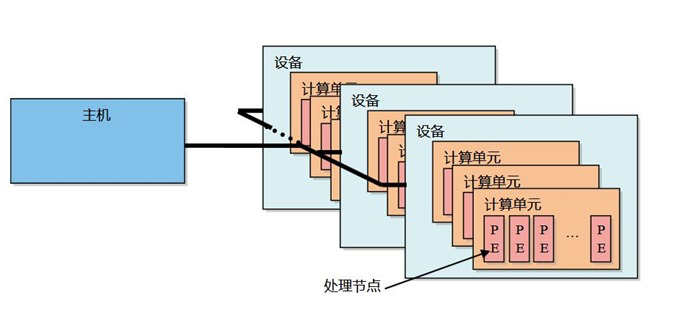
\includegraphics[width=4.8in,height=2.3in]{pic/opencl-host-device.png}
\caption{OpenCL的平台模型--host~\&~device模型}
\end{figure}

\paragraph{平台模型} 该模型描述内部单元之间的关系。主机(host)可以是个人计算机或超级计算机。OpenCL设备(device)可以是CPU 、 GPU 、DSP或其它处理器。每个OpenCL设备包含若干计算单元(compute unit ,CU),每个计算单元又由若干处理单元(processing element ,PE)组成。 \n
OpenCL通过平台实现主机与设备间的交互操作。主机管理着整个平台上的所有计算资源,所有OpenCL应用程序都是从主机端启动并在主机端结束的。应用程序运行时由主机提交命令(command),在设备上的处理单元中执行计算。每个计算单元内所有的处理单元都会执行相同的一套指令流程。每个处理单元以单指令多数据SIMD或单程序多数据SPMD模式运行指令流。 \n
然而,一般而言,选定了一个平台,那么就只能在这个平台所支持的设备上作计算了。用了Intel SDK就只能够用Intel的CPU进行计算,用了APP SDK就只能在AMD的CPU和GPU上进行计算。而且,一般两个不同的平台间时不能进行通信。

\paragraph{执行模型}OpenCL执行两类程序:内核程序(kernel)和主机程序(host program);前者由若干个OpenCL设备执行,后者由主机执行。OpenCL通过主机程序定义上下文(context)并创建一个被称为命令队列(command-queue)的数据结构来管理内核程序的执行。在命令队列中,内核程序可顺序执行(In-order Execution)也可乱序执行(Out-of-order Execution)。 \n
每当主机提交内核程序到设备上执行时,系统便会创建一个N维(N可取1,2,3)的索引空间NDRang。内核程序将索引空间中的每一点用一个工作项(work-item)来表示,将若干个工作项划分成一个工作组(work-group)。在一个计算单元内可运行同一个工作组中的工作项,并且该组内的工作项可以并发执行在多个处理单元上。 \n
执行模型可以进而再划分为内核,上下文,命令队列.

\begin{enumerate}
\begin{figure}[htbp]
\centering
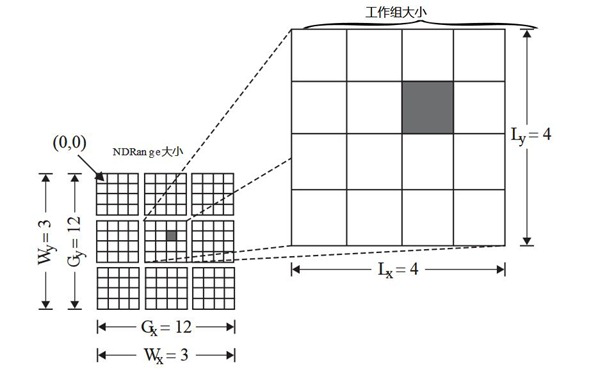
\includegraphics[width=4.8in,height=3in]{pic/opencl-kernel.png}
\caption{OpenCL's kernel}
\end{figure}
\item 内核 : 内核是执行模型的核心,它执行在设备上。在执行内核之前,需要先指定NDRange(N维度的范围)。NDRange是一个一到三维的index。这个index里节点的总f数目记为全局工作节点数。把全局工作节点分组,我们可以方便地管理各个节点。\n
全局工作节点数=工作组数 $\times$ 工作组中节点的数目。如图1.5,一共包含144个节点,分为9个工作组,每个工作组包含16个节点。 \n 
通过指定合理的节点数、工作组数,我们可以提高程序的并行度。
\item 上下文 : 一个主机要使得内核运行在设备上,必须要有一个上下文来与设备进行交互。 上下文是一个抽象的容器,用来管理在设备上的内存对象并且跟踪在设备上创建的程序和内核。主机通过上下文来与设备交互,使得内核运行在设备上。
\item 命令队列 : 每个设备都有一个自己的命令队列,而主机则负责把命令发送到对应设备的命令队列上。命令队列对在设备上执行的命令进行调度。在主机和设备上,命令是异步执行的。
\end{enumerate}

\paragraph{内存模型}
\begin{enumerate}
\begin{figure}[htbp]
\centering
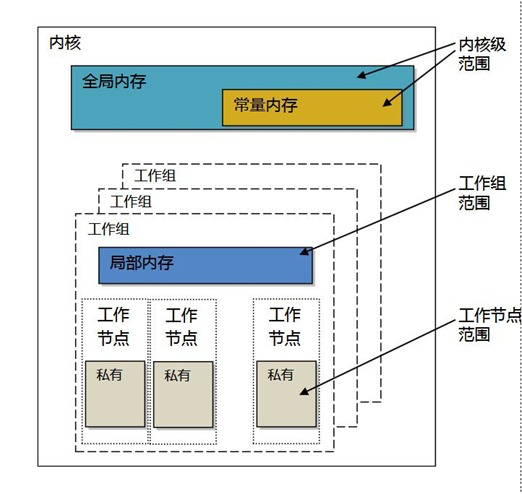
\includegraphics[width=4.8in,height=4.8in]{pic/memory.png}
\caption{OpenCL的内存模型}
\end{figure}
\end{enumerate}
OpenCL把内存模型抽象化了,通过这样来方便用户编写程序。在图1.6中,内存的分类如下:
\begin{itemize}
\item 全局内存 :所有节点都可以对其进行读写。
\item 常量内存 :全局内存中的一块区域,在内核的执行过程中保持不变。 由主机来负责分配和初始化其中的内存对象。
\item 局部内存 :由一个工作组里各个工作节点共享的内存区域。在OpenCL设备上,它可能会作为一块专有的内存区域存在,也可能会被映射到全局内存中。
\item 私有内存:仅属于一个工作节点的内存区域。
\end{itemize}

\paragraph{编程模型}
数据并行和任务并行是OpenCL可以支持的两种并行编程模型,同时两者的混合模型也得到支持。通常情况下,OpenCL采用的首要模型是数据并行,而对多核CPU主要采用任务并行。\n
数据并行编程模型中,一系列的指令会作用到内存对象(memory obect)的多个元素上。严格来说,数据并行要求内存对象单元与工作项保持一对一的映射,而在实际应用中,并不要求严格按照这种方式。在数据并行编程模型中,OpenCL又提供了一种分级方式,有两种方法:显式分级模型和隐式分级模型;前者要求开发人员指出工作项的总数和工作项所属的工作组;而后者仅需要开发人员定义工作项的总数,对于工作项的划分则根据OpenCL的实现来管理。在任务并行编程模型上,每个工作项都相当于在一个单一的计算单元内,该单元内只有单一工作组,该工作组只有该工作项本身在执行。

\paragraph{OpenCL软件框架}OpenCL软件框架包含三部分:OpenCL平台层、OpenCL运行时和OpenCL编译器。在OpenCL平台层上,开发人员可以查询系统中的平台数目并选定运行平台,在指定的平台上选择必要的计算设备并对它们进行初始化,然后可以建立上下文, 并创建命令队列。执行内核程序、读、写及复制缓冲区和同步操作等都是通过命令队列中的命令实现的。一个命令队列和一个OpenCL设备是一对一的关系。在OpenCL运行时中,开发人员建立内核实例,并将其映射到正确的内存空间中,接着在命令队列中排队执行内核。OpenCL编译器负责编译运行在设备上的程序,并创建可执行程序。

\paragraph{OpenCL实现原理}

从编程的角度来说, OpenCL中的操作都是和一个给定的上下文环境有关, 每个上下文环境中都有若干个相关的设备。在上下文环境中, OpenCL能够保证设备之间的内存一致性。OpenCL使用buffers(1维的内存块)和images(2维和3维的内存块)来存储内核数据。一旦分配了存放内核数据的内存空间, 并且指定了运行内核程序的设备,就需要装载和编译内核程序。为了执行内核程序, 程序员必须建立一个内核对象(kernel object), 并且设置内核参数。之后,内核就可以在命令队列中排队执行了。通常情况下, OpenCL设计的大致流程为:
\begin{itemize}
\item 创建并初始化OpenCL设备和上下文环境,建立命令队列;
\item 创建并编译源程序,建立内核句柄;
\item 分配数据所需内存空间,并将数据复制到OpenCL设备上;
\item 设置内核参数; 
\item 执行内核程序;
\item 将计算结果从OpenCL设备复制到主机中;
\item 释放系统所占资源。
\end{itemize}

\subsection{MPI调研}

MPI 是一种消息传递编程模型并可以被广泛使用的编写消息传递程序的标准。它由一组库函数组成,在Fortran或C 的基础上扩展为一种并行程序设计语言。严格来说,MPI只是一个库,提供了应用程序的编程接口,方便Fortran77/90或C/C ++等编程语言直接对这些库例程或函数进行调用,实现进程间通信。

\subsubsection{MPI数据类型}
为了支持异构环境和易于编程,MPI定义了精确的数据类型参数而不使用字节计数,以数据类型为单位指定消息的长度,这样可以独立于具体的实现,并且更接近于用户的观点。对于C和Fortran,MPI均预定义了一组数据类型(如MPI\_INT 、MPI\_DOUBLE等)和一些附加的数据类型(如MPI\_LONG\_LONG\_INT等),这些与语言中的数据类型相对应。MPI 除了可以发送或接收连续的数据之外,还可以处理不连续的数据,如多维向量或类C 语言中的结构数据类型。为了发送不连续的数据,MPI定义了打包(pack)与解包(un-pack)操作,在发送前显式地把数据包装到一个连续地缓冲区,在接收之后再从连续缓冲区中解包。MPI 还允许发送和接收不同的数据类型,使得数据重映射方便灵活。通过使用不同的数据类型调用MPI\_SEND ,可以发送不同类型的数据,使得MPI 对数据的处理更为灵活。

\subsubsection{通信域}
通信域是MPI的一个关键概念,它以对象形式存在,作为通信操作的附加参数。通信域为开发消息传递程序提供了模块化支持,从而强有力地支持开发并行库和大规模代码。MPICH 中的一个通信域定义了一组进程和一个通信的上下文,虚拟处理器拓扑、属性等内容。通信上下文是通信域所具有的一个特性,它允许对通信空间进行划分,提供了一个相对独立的通信区域,由系统严格管理,对用户是透明的,有力地保证了库代码的消息通信互不干扰。MPI\_COMM\_WORLD是一个由MPI提供的预定义的通信域,它包括所有的进程。所有的MPI实现都要求提供MPI\_COMM\_WORLD通信域,在进程的生命期中不允许将其释放。用户也可以在原有通信域的基础上,定义新的通信域。通信域为库和通信模式提供了一种重要的封装机制。

\subsubsection{MPI调用接口}
MPI-1提供了128个调用接口,MPI-2提供了287个调用接口,但MPI所有的通信功能可以用它的6个基本调用来实现,也就是说可以用这6 个基本调用来完成基本的消息传递并行编程。
\begin{enumerate}
\item MPI初始化:MPI\_INIT()是MPI程序的第一个调用,它完成MPI程序所有的初始化工作,也是MPI程序的第一条可执行语句。
\item MPI 结束:MPI\_FINALIZE()是MPI程序的最后一个调用,它结束MPI程序的运行,也是所有MPI程序的最后一条可执行语句。
\item 获取当前进程标识:MPI\_COMM\_RANK(comm ,rank)返回调用进程在给定的通信域中的进程标识号,有了这一标识号,不同的进程就可以将自身和其他的进程区别开来,实现各进程的并行和协作。指定的通信域内每个进程分配一个独立的进程标识序号,例如有n个进程,则其标识为0\~n-1。
\item 通信域包含的进程数:MPI\_COMM\_SIZE(comm ,进程通过这一调用得知在给定的通信域中一共有多少个进程在并行执行。size)返回给定通信域中所包括的进程的个数,不同的进程通过这一调用得知在给定的通信域中一共有多少个进程在并行执行。
\item 消息发送:MPI\_SEND(buf ,count ,datatype ,dest ,tag ,comm):MPI\_SEND将发送缓冲区buf中的count 个datatype数据类型的数据发送到目的进程dest,tag是个整型数,它表明本次发送的消息标志,使用这一标志,就可以把本次发送的消息和本进程向同一目的进程发送的其他消息区别开来。MPI\_SEND操作指定的发送缓冲区是由count个类型为datatype 的连续数据空间组成,起始地址为buf。
\item 消息接收:MPI\_RECV (buf, count, datatype, source,tag, comm.status)从指定的进程source接收消息,并且该消息的数据类型和消息标识和本接收进程指定的datatype和tag相一致,接收到的消息所包含的数据元素的个数最多不能超过count 。status是一个返回状态变量,它保存了发送数据进程的标识、接收消息的大小数量、标志、接收操作返回的错误代码等信息。接收到的消息的源地址、标志以及数量都可以从变量status中获取,如在C语言中,通过对status.MPI\_SOURCE, status.MPI\_TAG, status.MPI\_ERROR引用,可以得到返回状态中所包含的发送数据进程的标识,发送数据使用的tag标识和本接收操作返回的错误代码。
\end{enumerate}

\subsubsection{MPI并行编程模式}
MPI 具有两种最基本的并行程序设计模式:对等模式和主从模式,大部分并行程序都是这两种模式之一或二者的组合。并行程序设计的两种基本模式可概括出程序各个部分的关系。对等模式中程序的各个部分地位相同,功能和代码基本一致,只是处理的数据或对象不同。而主从模式体现出程序通信进程之间的一种主从或依赖关系。并行算法是并行计算的核心,用MPI 实现并行算法,这两种基本模式基本上可以表达用户的要求,对于复杂的并行算法,在MPI中都可以转换成这两种基本模式的组合或嵌套。

\paragraph{主从模式}
主从模式又称为 Master/Slave 模式,在这种模式的并行程序中,存在一个单独执行控制程序的主进程(Master),负责任务的划分、分派、结果的收集,负责所有进程间的协调和网络调度,并且在其它结点机调用Slave 程序等.执行从程序的若干进程称为从进程(Slave),负责子任务的接收、计算和结果的发送.\n
在这种模式下,一个程序由两部分构成:Master 程序和Slave 程序.主进程执行Master 程序,各子进程分别执行各自的Slave程序.主进程通过消息传递通信函数完成与并行处理机节点上运行的各子进程间的数据传输.Master 程序和Slave程序各自的程序框架如下:
\begin{figure}[htbp]
\centering
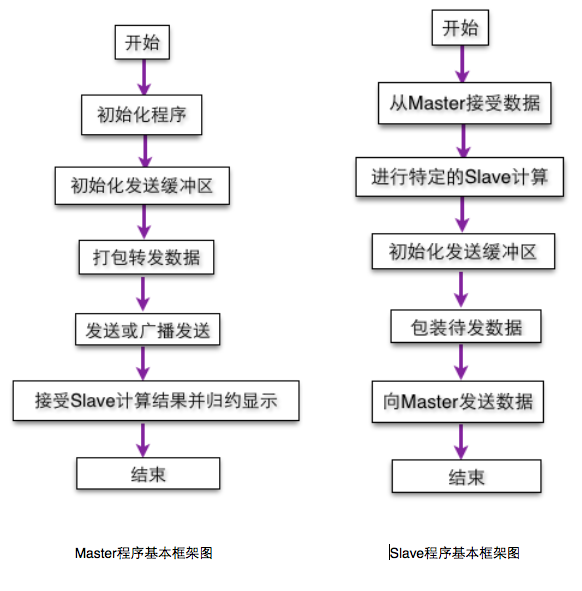
\includegraphics[width=4.8in,height=5in]{pic/MPI-master-slave.png}
\caption{MPI主从模式}
\end{figure}

\paragraph{对等模式}
对等模式又称为 SPMD 模式,在这种模式的并行程序中,各个部分地位相同,所有进程执行同一个程序,只是各进程计算的数据不同,控制和处理都在计算节点上. 各节点使用消息实现同步或异步通讯.对等模式程序基本框架如下:
\begin{figure}[htbp]
\centering
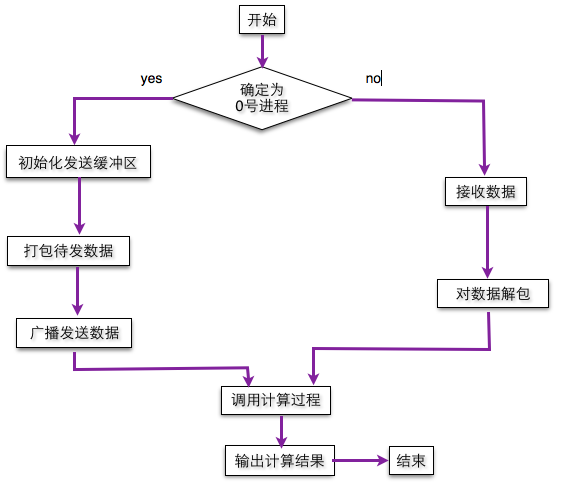
\includegraphics[width=4.8in,height=5in]{pic/MPI-equal-mode.png}
\caption{MPI对等模式}
\end{figure}


\subsection{想法来源及可能遇到的挑战}
并行计算如果按照硬件环境进行分类,那么以分布式计算为基础的计算机集群使其中典型的一类.以上三种并行框架大多是跨平台的,而inferno自身却具有分布式系统和以“资源皆文件”的优势,使得并行计算框架的构建更具有可执行性,但这个方向还鲜有相关研究.\n

根据相关调研,我们可能会面对下述问题 : 
\begin{enumerate}
\item 计算机集群实现分布式运算的特点,计算过程不一定是同步的,所以负载均衡是一个有挑战的问题,对应解决方案有Round-robin DNS,scheduling algorithms等.
\item 由于分布式计算需要共享实时数据,对于网络带宽以及低延迟网络的需求也是其需要考虑的问题,可以运用更高效率的传输媒介来处理.
\item 因为考虑的是并行框架,各个计算机、各个数据以及各个指令之间的竞争需要处理.例如:当计算机尝试覆盖相同或者旧的数据,而此时就的数据仍在被读取.结果可能是下面的一个或者多个情况:机器宕机、出现非法操作并结束程序、错误的读取旧数据、或者错误的写入新数据.在这里,竞争的危害出现于通过访问同一个信息通道的数据.解决的方法可以通过标记正在处理的数据以及标记读写来处理.   
\item 分布式系统中的另一个问题是容错性问题(fault-tolerance).这也是有名的拜占庭将军问题(Byzantine failures).在容错的分布式计算中,拜占庭失效可以是分布式系统中算法执行过程中的任意一个错误.这些错误被统称为“崩溃失效”和“发送与遗漏是失效”.当拜占庭失效发生时,系统可能会做出任何不可预料的反应.这些任意的失效可以粗略地分成以下几类;进行算法的另一步时失效,即崩溃失效:无法正确执行算法的一个步骤;执行了任意一个非算法指定的步骤.具体来说就是所写的并行框架在没有容错处理时出现让人匪夷所思的随机错误.具体可以通过口头消息算法或签名消息算法解决.
\end{enumerate}
 

\section{可行性研究报告}

\subsection{理论依据与技术依据}

\subsubsection{Sytx协议及其具体实现}

Inferno的文件系统协议(或Sytx)是贝尔实验室九号项目所开发的针对于分布式操作系统的网络协议,作用是链接系统内的组件.Inferno系统中文件是核心,这些文件代表了视窗、网络连接、进程、以及其他存在于操作系统中的各种元素.不同于NFS,Styx的用途是把数据缓存起来,并提供虚拟文件的机制(例如/proc用以表示进程).\n
在Inferno系统中,Inferno服务器(Inferno server)是被用来被Inferno进程访问的并提供分等级文件系统(文件树)的代理.一个服务器响应客户端的请求并导引文件树中的具体位置,同事可以对文件进行创建、删除、读写等操作.\n
对于某个服务器来说,连接是通过一个客户端和服务器间的双向的通信通道来实现的.客户端可能是单一的,也可能有多个客户共享同一连接.一个服务器文件的文件树通过bind和mount命令联结到一个进程组的命名空间上.这样,组内进程就是服务器的客户端:对于文件的系统调用就被翻译为请求和响应,并得到相应的服务.\n 
      Inferno的文件协议,Sytx,就是用于处理客户端和服务器间的消息(message)的.目前我们组所用的Sytx版本是和9P2000一致的.客户端给服务器传递请求(T-messages).相应的,服务器返回响应给客户端(R-messages).这样就构成了基本的发送和接收机制.关于message的样式,这里就不再赘述.不过值得一提的是fid——一个客户端用来辨认服务器上当前文件的32位无符号整型.\n 
      Styx在客户端及服务器端提交如下的消息.这些消息对应到虚拟文件系统层的进入点,所有的服务器都必须实现这些消息:
\begin{enumerate}
\item version : 交涉协议的版本.
\item error : error.
\item flush : 终止消息.
\item auth, attach : 打开连接.
\item walk : 走访目录层次结构.
\item create, open : 准备一个用来写入/读取既有或新增文件的fid.
\item read, write : 发送数据给文件或从文件接收数据.
\item clunk : 抛弃fid.
\item remove : 从服务器移除文件.
\item stat, wstat : 查询或变更文件属性.
\end{enumerate}
这些具体实现中,有几个是我们工程的技术依据:
\begin{enumerate}
\item walk message : walk消息使得服务器变更当前的与fid相联系的文件为一个在目录中旧的“当前文件”或者某一个它的子目录.Walk返回一个新的fid,这个fid指向于该文件.通常,客户为根目录保留fid,然后通过walk从根fid进行导引.
\item attach,auth message : attach消息用来从客户端的用户向服务器提供一个连接点(introduction).这条消息识别用户并选择文件树去访问.attach消息会使客户端会拥有一个指向目标文件树根目录的连接,当然这个目录通过fid来被识别.Auth消息包含一个afid,用来进行认证.一旦认证协议完成,相同的afid会被attach提供给用户来保证成功进入并获取服务.
\item stat,wstat :stat消息获取文件信息.Stat字段包括文件名,读写、执行权限,访问和修改次数,所有者和组的信息.Wstat允许默写文件的属性被做某些改动.
\item flush : flush信息可以终止某个请求.当服务器收到 Tflush,它就不会回复带有oldtag标记的消息并立刻发送Rflush.客户端必须等待直到得到Rflush.这时oldtag会被回收.
\item write,read,open,create,remove功能都如上面简介介绍.
\end{enumerate}
~\n  另外,Styx对于安全性也做了一定工作,提供了许多安全机制来处理会影响系统整体性和安全性的危险动作.统一的文件通信协议包含着用户和组的识别码.比如,在收到一个打开文件请求时,服务器会检查并匹配用户id.这个机制和通用操作系统比较类似.Styx用通过网路连接的文件系统方式提供远程资源.这种获取远程资源的方式对应用程序是透明的,所以认证不需要特别提供.例如,在inferno中,客户端和服务器间的通信渠道中会包含许多加密和消息摘要的协议.与通用文件服务器和一些电话通讯领域一样,所有对于资源的运用都会经过一定的认证,这也保证了远程管理的安全性.\n
  值得一提的是Styx协议将请求翻译为必要的字序列并将其在通信通道中传递.所以Styx协议适应于ISO标准的OSI Session Layer Level.所以它独立于机器结构并成功地应用于不同指令集和数据格式的机器中.

\subsubsection{ns - 显示当前命名空间}
 在立项依据中,我们简要介绍了命名空间的概念,在Inferno系统中,命名空间是一系列挂载点(mount points)和绑定(binds)的集合,与UNIX系统的挂载点相似.在Inferno系统中,你可以把一个使用styx协议的服务器挂载在一个文件描述符上(如一个网络连接,或者一个程序的管道),因此,挂载在命名空间中引入了一个新的文件树;另一方面,挂载还可以仅仅使命名空间的一部分作为一个别名出现在另一个命名空间中.\n
命名空间包括两个部分:常规路径,以“/”开始;和一个“特殊”的路径集合,以“\#”开始,后面跟单个字符.这些特殊路径是内核设备,为内核服务的文件树,频繁访问的硬件(如硬盘)或者内核数据结构(如处理器).只有命名空间中的常规路径可以通过bind、mount、unmount指令修改.ns命令用来打印当前的命名空间,在shell中执行ns命令打印出的是shell的命名空间.为了举例说明,下面是在初始Inferno下运行ns的输出:

\lstinputlisting{result/ns} ~\n
 如上面的输出所示,大多数行在常规文件系统中bind一个内核设备,例如\#U(Inferno根目录的内容)在/,\#m(鼠标)在/dev上,\#I(网络栈)在/net上.-a和-b选项分别表示第一条路径的内容出现在原来第二路径的后面和前面(第二条将会包含第一条路径和它自己的集合).如果出现选项-c,目标路径将允许文件创建.上面出现的命名空间是被Inferno初始化代码安装的,作为一种引导系统的方式给出一个合理的默认命名空间.
\n
挂载在命名空间中引入了一个外部文件树,就像UNIX系统mount一样,文件树被文件描述符上使用styx协议访问.内核通过翻译open/read/write/stat/stc系统调用成styx信息来控制styx部分,然后在返回值中回复信息.mount系统调用要求文件描述符使用styx协议通信.mount程序挂载3种类型的styx服务器拥有很方便的语法:

\begin{itemize}
\item mount /path/to/styx/file target, 通过打开/path/to/styx/file取得文件描述符
\item mount net!www.example.org!styx target, 通过访问net!www.a.org!styx取得文件描述符
\item mount {program} target, 开始程序并且用它的标准输入作为文件描述符
\end{itemize}

ns显示给定pid或者默认它本身的命名空间结构,以/prog/pid/ns的内容为基础,打印一系列bind和mount命令,如果它被执行,会重建一个相同的命名空间.如果任何涉及到的文件因mount或bind命令被改名,那么就显示文件的原始名字.

\subsubsection{bind, mount, unmount - 修改命名空间}

  bind和mount命令修改当前进程和在一个命名空间组中其他进程的命名空间,目标是一个存在的文件或当前将要修改的命名空间的目录名.对于bind,目标是一个已经存在的文件或当前命名空间下的目录名.在bind命令成功执行之后,目标文件名就是原来的东西起的一个别名;如果修改没有隐藏它,目标将依然指向他的原来的文件.源和目标必须是同一个类型,要么都是目录,要么都是文件.对于mount,源可以是一个shell命令,一个网址,或者一个文件名,如果源被花括号扩起来,那么它将作为一个sh命令的调用,如果源中包含感叹号或者没有文件,他将被作为一个网址.
\n
 bind和mount命令的工作可以被unmount命令撤消,如果给unmount两个参数,他会撤消相同参数的bind或mount命令,如果只给它一个参数目标上所有bind过和mount过的东西都会被撤消.注意,当使用bind或unmount命令时,内核设备名称中的\#字符必须被引号引起来否则shell会把它看做注释的开头. \n
修改命名空间的常用选项:
\begin{itemize}
\item  -b : mount和bind均有效.把源目录加入被目标目录代表的联合目录开头.
\item  -a : mount和bind均有效.把源目录加入被目标目录代表的联合目录结尾.
\item  -c : 这个选项可以加在上面两个选项上,用来允许在联合目录中的创建.当在联合目录中创建一个新的文件时,它将被放在联合目录中第一个mount或bind带有-c选项的元素中,如果那个目录没有写权限,将会创建失败.
\item  -q : 如果bind或mount失败,不打印诊断信息,安静退出.
\item  -A : 只对mount有效.在执行mount之前不认证服务连接.
\end{itemize}

\subsubsection{os - 寄主操作系统接口(对寄生安装的Inferno有效)}
os指令将使得我们使用C语言开发的程序在Inferno系统中运行.\n
  os使用使用cmd设备在寄主系统执行命令,如果存在-m选项,os会使用在挂载点的设备,否则将会被假设在/cmd下,如果必要还会被bind在本地命名空间下.-d选项将会导致命令运行在dir目录下,如果dir目录不存在或者无法访问就会报错,且指令不会执行.命令的标准输出和标准错误会出现在os命令本身的标准输出和标准错误上,os复制标准输入到远程命令的标准输入;如果命令没输入,就会重定向os的输入到/dev/null.当cmd终止后,os命令就终止了,它的退出状态返回的是cmd的退出状态.如果命令被杀死或退出(比如缺少输入或输出),寄主自己的进程控制办法将试图杀死仍在运行的cmd,-b(background)选项将制止这个行为.-n选项导致cmd在低于正常优先级下运行.-N选项把低优先级设置为特殊的等级,从1到3.

\subsubsection{cpu - 执行一个远程的命令}
cpu命令向主机拨号(使用tcp网络如果网络没有显式给出).连接后,向外传输本地的命名空间并执行远程机器上的指令.本地命名空间对于/n/client中的命令是可见的;本地的设备文件被bind到了远程设备目录下.如果命令没有给出,那么/dis/sh就处在运行之中. \n
-C选项设定了authentication被摘要或者加密的算法,具体的摘要算法有:MD4,MD5等,具体的加密算法有:RC4,DES,CBC,ECB等算法.默认的是不用任何算法.

\subsubsection{file2chan - 节点间通讯}
因为我们要实现并行计算框架,一个亟待解决的问题就是如何做节点间通讯.最初我们的想法是直接用一个文件来做共享池.然而后来在此基础上进行实现时发现困难重重:
\begin{enumerate}
\item 直接用文件做共享难以解决同步的问题.因为直接用文件做共享池,这样在运行时没法动态的加锁,解锁,不方便解决同步问题.
\item 难以实现主节点的动态任务分配.
\item 难以实现主节点对从节点请求的动态响应.
\item 光是一个文件难以做到传输各种格式不同的通讯信息.
\item 直接在磁盘中暴露中间计算内容,缺少加密.
\end{enumerate}
~\n
经过我们重重调研,发现Inferno提供了一个叫做file2chan的脚本工具.\n
file2chan是一个sh的可加载模块,可以在命名空间中创建一个可以由shell脚本决定其性质的文件.file2chan在命名空间中创建一个文件名,同时产生一个新的线程来为这个文件服务,如果成功了,环境变量\$apid就会被设置成新线程的pid,否则返回一个错误状态(non-nil).readcmd、writecmd和closecmd都应该是可执行的指令块.之后,每当一个进程从文件名读入,就会调用readcmd;每当一个进程对文件名写入,就会调用writecmd;每当一个从文件名打开的文件关闭,就会调用closecmd.\n
如果我们采用file2chan,则可以轻松的解决上述问题.具体设想与实现可以参考概要设计报告部分.

\subsection{创新点}

\subsubsection{良好的异构支持}
由于Inferno的分布式特性.我们的并行框架具有天然的跨平台性,可以实现arm, x86, amd64节点混合成的混合集群.\n
同时我们借鉴了OpenCL的平台模型,并采用抢占式任务分发以及细并行粒度的任务分配,可以使得计算能力相差很大的节点协作计算.具体内容可以参见概要设计报告中异构的部分.

\subsubsection{实现MapReduce计算模型}
尚未有人、或极少人在Inferno上做过并行计算.然而,Inferno系统本身的特性使得它能很方便的实现并行计算.为了进一步完善我们小组的并行计算模型,我们也在Inferno上实现了MapReduce这一编程模型.通过MapReduce, 我们可以把一个大作业拆分成多个小作业,而用户只需要决定拆分成多少份,以及定义作业本身.因此,不熟悉并行编程的程序员也能充分发挥分布式系统的威力.事实证明,Inferno在实现并行计算框架这一点上较其它系统有天然的优势,只要进行少量的工作就完成了MapReduce在Inferno上的移植.

\subsubsection{多节点视为整体的一个节点}
集群是一组相互独立的、通过高速网络互联的计算机,它们构成了一个组,并以单一系统的模式加以管理.如今主流的集群实现方式中,集群中节点间的数据交换通过数据共享空间或者点对点的通信实现,各个节点事实上并不能真正成为一个整体,例如基于MPI(Message Passing Interface)的并行框架.而inferno通过导入Namespace(命名空间),使所有的资源都以分层次的文件的形式存在于文件系统中,因此应用程序可以以同样的方式访问远程的节点和本地节点.故而虽然这个系统上包含了很多的节点, 但是在用户和应用程序看来, 这就像是一个节点一样. 

\subsubsection{Inferno在64位平台上的移植}
最新的inferno第四版发行于2004年,支持的平台有ARM,PA-RISC,MIPS,PowerOC,SPARC,X86.但如今市面上的平台基本上都是64位的了,因此要想在64位的平台上运行inferno,就要进行移植.为了让Inferno能成功地在市面上绝大多数电脑上运行,把更多的平台纳入我们的并行框架中,我们修改了Inferno的部分代码,将其移植到了64位的平台上.

\subsubsection{以外部解释器的形式实现并行计算}
之前调研了其他著名并行计算框架的使用方式:
\begin{itemize}
\item CUDA, MPI : 用户根据具体的MPI实现框架(Intel MPI, OpenMPI等)给定的API接口,调用具体的库函数,进行串行代码的并行化移植.
\item OpenMP : 在要并行的代码块前加预处理指令\#pragma.编译器编译时则自动会链接OpenMP库,编译出并行化代码.
\end{itemize} 
~\n
我们借鉴了OpenMP的并行化的技术,提出了使用外部解释器思想.我们是针对Inferno的shell实现并行计算框架,而shell并不需要编译,是通过Inferno中自带的sh逐行解释执行的.然而直接对Inferno中的sh动手脚是不可能的,sh部分代码量高达好几万行,没有注释并且还使用了部分内核接口.我们之前调研发现Inferno的shell本身就自带bind, cpu, file2chan等工具,可以直接编写能在Inferno的shell上运行的并行化代码.所以我们决定实现一个外部解释器,将用户的串行代码按照给定的需求解释成能直接在Inferno的shell中直接运行的并行化代码.\n

这点和OpenMP又有极大的不同,OpenMP并行化的程序在运行时还需要调用OpenMP库.而我们则要实现串行代码再经过解释器解释之后可以直接在Inferno的sh上运行,不需要再调用其他库,可以说是得到了在Inferno平台下“完全并行化”的代码.

\subsubsection{以C语言而非Limbo语言来编写解释器程序}
在Inferno里,我们需要用Limbo来写应用程序.Limbo是一种用于分布式系统的编程语言.然而Limbo是一门不流行的语言,相关文档较少,因此学习这门语言势必需要花费较多的时间与精力.但是,假如我们是以应用程序的形式在别的系统上运行Inferno,那么我们就可以通过os这条命令,来间接地在Inferno上运行host机器上的程序.于是,我们小组选择了用C语言来写解释器,通过os命令来间接地让解释器在Inferno上运行,大大加快了开发进度.

\subsubsection{对file2chan的读写方法封装,实现一个文件完成各种类型通讯}
此部分具体见概要设计报告中的sharedPool - 节点间通讯一节. 


\section{概要设计报告}

\subsection{总体路线}
在理论依据部分和创新点部分已经提及了我们的部分设计思路.我们的最终目的就是实现一个外部解释器,可以根据需求将用户给定的串行程序翻译成基于host~\&~device模式的,可以在Inferno的shell环境下直接运行的并行化代码. \n
总的开发阶段可以划分为如下两个部分:
\begin{itemize}
\item 自己先摸索出在Inferno中将串行程序并行化改写的方法,并对具体语句总结出一套模式化改写规则(如对一段for改如何改写)
\item 开发解释器,按照之前总结的改写规则将串行代码翻译为并行代码.
\item 在Inferno在x86/64的机子上完成部署.并将Inferno移植到Raspberry Pi上,搭建通过局域网互联的跨架构的集群.
\item 在搭建的集群上测试我们解释器,完成最终部署.
\end{itemize}
~\n

\subsection{平台模型 - OpenCL的host~\&~device模式}
根据我们之前对常见并行计算框架的调研以及Inferno的架构,我们最终决定选用Opencl所用的平台模型 - host~\&~device模型作为我们的平台模型. 原因如下 : 
\begin{itemize}
\item host~\&~device模式非常成熟.当前最为流行的支持异构的并行计算框架OpenCL和CUDA都采用它作为自己的平台模型
\item 在host~\&~device模式中,host就像一个大管家,完成任务调度,节点通讯,负载均衡功能.因此device则只需care自己那部分的运算即可,无需care自身目前所处的环境.即实际运行环境对device是不可见的,device不需要对运行环境的变化做出变化.这一点对于异构是至为重要的.
\item Inferno的架构非常适合采用host~\&~device模式.根据前期对Inferno的namespace和styx的调研,我们可以简单的用bind的命令将远程的Inferno节点的资源挂载在本地,亦或是用cpu命令直接在远程端运行给定程序.所以可以选择一台节点作为host,其余节点作为device.然后将device全部挂载在host上.由host分发任务,响应device请求,进行device间调度等.采用这种平台模型可以大大推进我们开发速度.
\end{itemize}

\subsection{异构性}
首先,我们采用了OpenCL和CUDA所使用的平台模型 - host~\&~device模型作为我们的平台模型,奠定了异构基础.\n
为了进一步支持,我们提出了细并行粒度和抢占式任务分配的观点.

\subsubsection{抢占式任务分配}
为了更好地支持异构,我们决定采用抢占式任务分配的方式.在这种方式下,host无需主动分配任务给device,而是将下一个任务放在共享池中让已经完成了之前任务的空闲device来抢占.当前共享池中的任务被抢占后,host根据计算情况再将新的任务放在共享池中.

\subsubsection{细并行粒度}
在并行计算中,并行粒度 = 计算量 / 通信量。计算和通信交替出现,两者通过同步时间相区分。并行粒度受限于应用程序算法的内在特性。由于选择正确的并行粒度有助于程序暴露更多的可并行性,因此为了充分发挥基础平台的性能,选择正确的并行粒度非常重要.选择合适的并行粒度可以提高并行化加速比。经过调研我们得到如下结论 : 

\paragraph{细粒度的并行}
\begin{itemize}
\item 计算强度低
\item 没有足够的任务来隐藏长时间的异步通信
\item 容易通过提供大量可管理的(即更小的)工作单元来实现负载均衡
\end{itemize}

\paragraph{粗粒度的并行}
\begin{itemize}
\item 计算强度高
\item 完整的应用可以作为并行的粒度
\item 难以有效实现负载均衡
\end{itemize}

根据上述结论,我们决定采用细并行粒度.对于每个device,由于并行粒度细,各个device之间同步需求不大,且每次由host分配给它的任务并不繁重,可以在较短时间计算完成.再由抢占式任务分配机制,计算完成的节点把结果提交给host之后可以直接从host中抢占任务,而不是等待其余device. \n
如此实现,在一定程度上可以避免计算能力低的节点拖累计算能力高的节点,从而提高了异构性.

\subsection{Raspberry Pi2}
Inferno强调的是分布式,适用于多种架构,从pc到嵌入式系统.所以在设计并行框架时应该利用Inferno这一强大的特性实现对异构的支持.于是搭建Inferno集群时,我们准备安排一个arm架构的结点.\n
\begin{figure}[htbp]
\centering
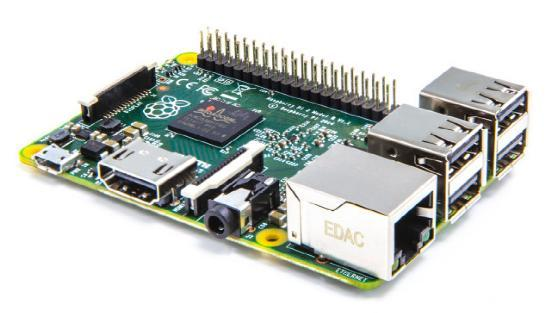
\includegraphics[width=4.8in,height=2.3in]{pic/raspberry-pi.jpg}
\caption{Raspberry Pi2}
\end{figure}

经过调研论证,我们决定选择Raspberry Pi2作为arm节点.\n
Raspberry Pi是一款基于Linux系统的只有一张信用卡大小的单板机电脑。它由英国的树莓派基金会所开发,目的是以低价硬件及自由软件刺激在学校的基本的电脑科学教育。\n
2015年2月,树莓派基金会发布了第二代产品 - Raspberry Pi2,售价35美元。Raspberry Pi2采用4核Broadcom BCM2836 (ARMv7-A)芯片、双核VideoCore IV GPU和1GB内存,\n

\section{理论研究与实践}
纸上得来终觉浅,绝知此事要躬行.我们组经过反复论证探讨之后,开始实践工作.

\subsection{Inferno在Raspberry Pi移植}
根据前期调研,我们决定采用hosted方式在Raspberry Pi上运行inferno.刚好组长阮震元所在的ACSA实验室里有空闲的树莓派可以使用.\n
首先我们在自己的电脑上搭建了arm的交叉编译工具链条.根据Raspberry Pi的情况我们采用了armv6j-hardfloat-linux-gnueabi.完成了arm-glibc, arm-gcc等交叉编译环境的部署. \n
接着即为针对Raspberry Pi的环境对inferno源码做了11处修改,使得原版的Inferno与Raspberry Pi配适. \n
进行的过程中遇到了各种困难,例如Inferno原版的setfcr-Linux-arm.c已经过时了,在使用4.7以上的arm-gcc会遇到错误,需要对其根据编译环境做相应调整,又如Inferno的styx协议无法在Raspberry Pi上正常运行,最终定位到内核AF\_INET模块,需要对内核配置进行修改. \n
 在移植的过程中,我们还积极联系了Inferno的官方开发组,和他们共同完成这项工作.在此阶段组长阮震元还向Inferno官方上报了2个Inferno在arm下的bug,均引起重视.一个被官方列为major等级\footnote{https://bitbucket.org/inferno-os/inferno-os/issue/326/arm-listen-failed-because-ipv6-support-is},另一个则被官方列为critical等级\footnote{https://bitbucket.org/inferno-os/inferno-os/issue/325/arm-build-failed}.阮震元还针对Inferno在amd64下编译问题向官方提供了一个有效的patch\footnote{https://bitbucket.org/inferno-os/inferno-os/issue/329/a-patch-for-x64}.\n
最终我们在Raspberry Pi上成功运行了Inferno!
\subsection{初步尝试 --- 一个串行程序}
\lstinputlisting{code/deviceSerial.sh}
~\n
先简要的解释一下这个程序.subfn fac实现了一个计算阶乘的子函数.subfn c实现了一个组合数的子函数.subfn calc实现了一个统计函数,对于给定的n可以统计有多少个$r\leq n$满足$C(n,r) > 1000000$.\n
最外层则是一个i从23到100变化的for循环,将所有的calc(i)相加输出.值得注意的是在Inferno下任何算数运算都采用后缀表达式并通过调用内嵌子函数expr完成.\n
本身这个程序没有任何意义,举这个程序为例子只是为了演示如何将一段串行代码并行化.

\subsection{初步尝试 -- 改写的host~\&~device式并行代码}
\paragraph{host部分}  
\lstinputlisting{code/host.sh}
\paragraph{device部分}
\lstinputlisting{code/device.sh}  

\subsection{file2chan - sharedPool的基础}
file2chan是user namespace下的程序,通过对Inferno内核的系统调用实现了内存中的虚拟文件。\n
file2chan接受2个代码块writecmd和readcmd作为参数。当用户读虚拟文件时则会执行readcmd中的代码,当用户对虚拟文件写时则会执行writecmd中的代码。\n
利用file2chan我们将虚拟出一个虚拟文件并进一步封装成一个sharedPool用来做动态的节点间进程通讯。\n
file2chan的代码如下
\lstinputlisting{code/file2chan.b}


\subsection{sharedPool - 节点间通讯(任务分配收发池)}
首先在host部分我们通过file2chan定义了一个虚拟文件/tmp/sharedPool用作节点间通讯.然而由于节点间通讯消息种类十分繁杂(例如主节点给从节点分配任务,从节点计算完毕将结果提交给主节点),各自的格式也都不一样.如果开多个file2chan则必定会带来管理的紊乱.于是我们创新性的采用封装了file2chan的read,write方法使得一个file2chan可以完成各种类型的信息通讯. \n
当想使用sharedPool进行消息通讯时,首先向sharedPool写入具体的操作类型.sharedPool中的我写好的read的方法会读取给定的操作类型,并在内部根据给定操作类型切换响应的模式来应对. \n
例如在我这个例子中,当device想要向host索求数据时先向sharedPool写入get,然后再对sharedPool执行读取操作即可读到主节点分配给它数据.当device计算完成,要把结果反馈给host时就先向sharedPool写入put,然后再往sharedPool写入算得的数据,此时就会触发sharedPool的write方法,自动将本次device向host提交的结果计入总结果.

\subsection{device部分代码}
并行部分的device代码和之前的deviceSerial的主要区别就是任务的分配方式不同。串行版的deviceSerial是自己决定计算任务,而并行版的device是向host抢占任务,待抢占到的任务计算完毕后则将结果放回sharedPool,而device则无需关心结果该如何统计这一切都由host完成,device只需再向host抢占任务即可。\n
由于已经对sharedPool做了高度封装,device只需简单调用即可。抢占任务由subfn getTask实现,提交结果由subfn writeRequest实现。

\subsection{host部分代码}
host部分主要实现了对sharedPool的封装。fn checkHost和fn readyHost负责启动各个device节点,使其进入pending状态。file2chan /tmp/sharedPool实现了对sharedPool的封装,内部的lock段代码再结合外部的subfn cannotWrite实现了对sharedPool的同步处理。

\subsection{并行框架开放的三个函数}

\subsubsection{map}
map函数即所谓的映射函数,其原型来自于函数式编程。而为了说明方便,我们用Python和Haskell中的map函数作为比对。对于Python,map函数需要两个参数,一个是某个函数f,另一个是一个可迭代的参数iterable(通常是一个数组)。当调用map(f, iterable)时,f会作用于iterable中的每一个元素并返回一个和iterable大小相同的数组result,result数组的每一个元素都是f作用于iterable对应元素的关于f函数的像,即result[i] = f(iterable[i]) .举个例子:

\begin{figure*}[htbp]
\centering
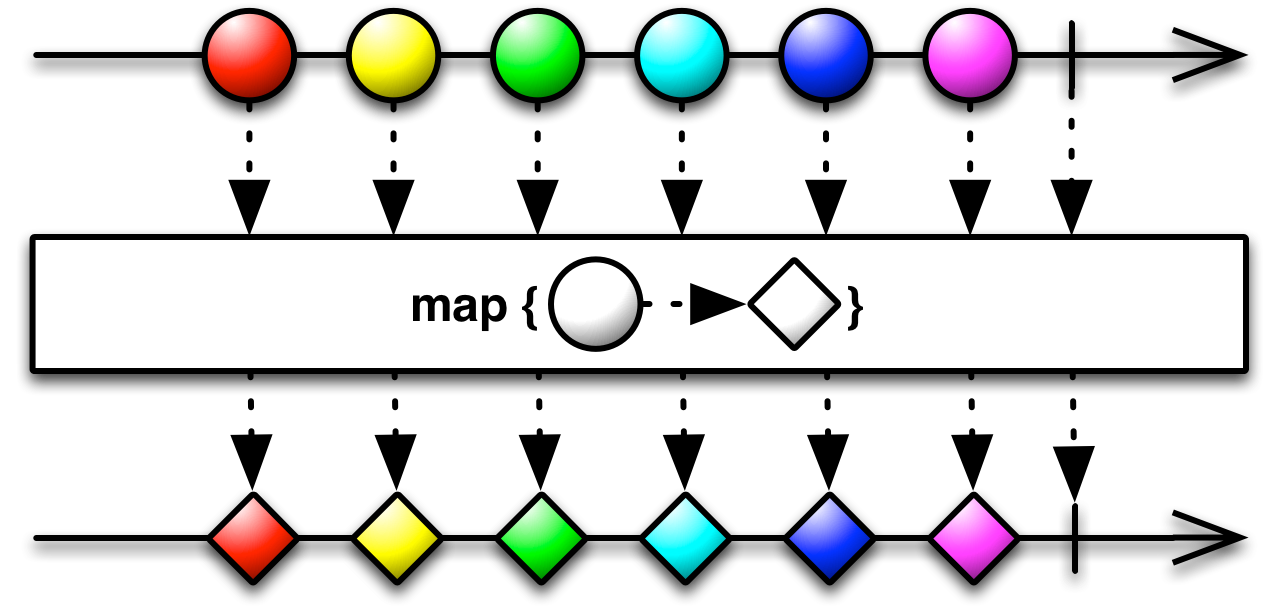
\includegraphics[width=\textwidth]{pic/map.png}
\caption{map函数示意图}
\end{figure*}


\begin{lstlisting}[language=python]
>>> def add100(x):
... return x+100
... 
>>> iterable = [11,22,33]
>>> map(add100,iterable)
result = [111, 122, 133]
\end{lstlisting}
不难看出,在一般情况下,在一般含义下,map函数可做如下解释:\n
map(f, iterable)<———->[f(x) for x in iterable] \n
对于Haskell,也是类似的: \n
map取一个函数和List做参数, 遍历该List的每个元素来调用该函数产生一个新的List. 看下它的类型声明和实现: \n

\begin{lstlisting}[language=haskell]
map :: (a -> b) -> [a] -> [b]
map _ [] = []
map f (x:xs) = f x : map f xs
\end{lstlisting}

我们小组采用了类似于Python中map函数的用法,并对其进行了并行化。作为用户视角,用户只需标示出并行符号@parallel\_begin,并且给出函数f和数组array,调用map函数,并且以@parallel\_end作为结束就可以得到并行化的代码。举个例子:

\begin{lstlisting}[language=shell]
subfn calculate {
    result = ${expr $1 1 +}
}
array1 = 120 121 122 123 124 125 126 127 128 129 130
@parallel_begin
map array1 calculate
@parallel_end
\end{lstlisting}

\subsubsection{reduce}

reduce函数是一种对满足结合律的函数f进行计算的函数。Python中的reduce内建函数是一个二元操作函数,他用来将一个数据集合(链表,元组等)中的所有数据进行下列操作:用传给reduce中的函数 func()(必须是一个二元操作函数)先对集合中的第1,2个数据进行操作,得到的结果再与第三个数据用func()函数运算,然后重复进行二元操作,直到最后得到一个结果。简单来说,可以用这样一个形象化的式子来说明:reduce( func, [1, 2,3] ) = func( func(1, 2), 3)。更为形象地看,我们可以用下图来分析。
我们小组的reduce函数用法是这样的:

\begin{lstlisting}[language=shell]
subfn funct {
    result = ${expr $1 $2 +}
}
input_list = 1 2 3 4 5 6 7 8 9 10 11 12 13 14 15 16 17 18 19 20 21 22 23 24 25 26 27 28 29 30 31 32
@parallel_begin
reduce input_list funct
@parallel_end
\end{lstlisting}

作为用户,只需要给出函数f,input\_list,标示出并行符号@parallel\_begin并且以@parallel\_end作为结束就可以得到并行化的代码,得到最后的结果。

\begin{figure*}[htbp]
\centering
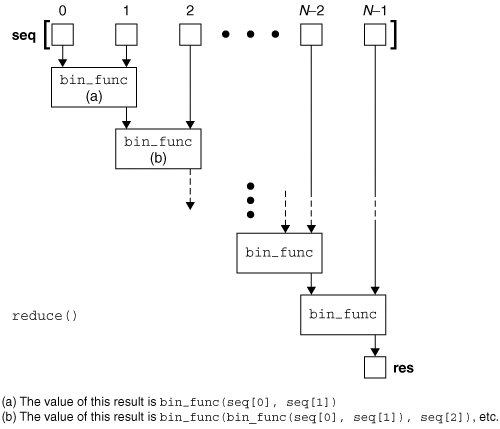
\includegraphics[width=\textwidth]{pic/reduce.png}
\caption{reduce函数的示意图}
\end{figure*}

\subsubsection{merge}

\begin{figure*}[htbp]
\centering
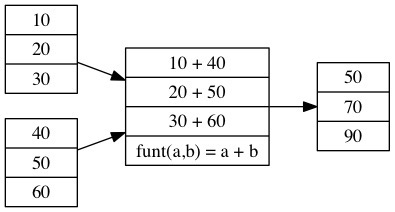
\includegraphics[width=\textwidth]{pic/merge.png}
\caption{merge函数的示意图}
\end{figure*}

merge函数是对多个数组或者表结构进行合并的函数。我们给出一个二元函数func,并给出两个数组list1,list2,当调用merge的时候,会返回另一个表list3。简单地讲,就是list3[i] = func(list1[i], list2[i])。更为形象地说,可由下图表示:

我们小组的merge函数用法是这样的:

\begin{lstlisting}[language=shell]
subfn funct {
    result = ${expr $1 $2 +}
}

input_list1 = ${expr 1 99 seq}
input_list2 = ${expr 99 1 seq}

@parallel_begin
merge input_list1 input_list2 funct output_list
@parallel_end
\end{lstlisting}

作为用户,只需要给出函数f,input\_list1,input\_list2,标示出并行符号@parallel\_begin并且以@parallel\_end作为结束就可以得到并行化的代码,得到最后的合并的表。

\subsection{函数并行化原理与容错机制}
    为了更好地体现分布式系统可靠性的特点,我们所做的并行计算框架考虑了容错问题,即当某些计算节点因为停机或网络中断而无法继续计算,并且无法与host交换数据的时候,要保证计算结果的正确性。为了实现故障的发现和处理,我们采取存储冗余数据的方法进行容错。

\subsubsection{map}
 对于map来说,冗余数据就是device的信息和device所抢占的数据,当device从host处获得要计算的数据时,host会在pool中留下冗余数据文件,文件名包含device所运行的计算进程的进程号client\_pid,用来区分不同的计算节点,文件的内容存储了获得的数据和其他信息,比如ip地址等,用来检测并处理故障。\n
    当host将任务分发完成后,pool中至少有一个刚刚发出的任务,可能还会有许多计算还没有完成,pool中还留有很多上述的冗余数据文件,此时仍然会有一些device上交计算结果,并试图获取新的计算任务,此时host并不终止该device的计算,而是从pool的冗余文件中挑选一个其它device还没有算完的任务分配给它,这样可以充分利用计算资源,避免忙等,从而减少故障修复所花费的时间。\n
    以这种方式分配出去的任务仍然要建立冗余数据文件,用来防止该device出现故障。此时剩余没有算完的数据可能有很多device在同时计算,他们之中也许有出现故障的节点,也许只是因为计算所需时间较长,计算还没有结束。但终究有一个时刻,最先完成计算的节点会向host提交数据,此时,host在清除该节点的冗余数据的同时,要检查pool中所有的冗余文件,凡是找到和该数据相同的文件,即表示获得了同样得到该任务的其它节点的信息,此时可以逐个在其中判断故障,判断这些节点与host网络的连通性,如果发现某个device无法和host通信,表示该节点出现故障,要把该节点的IP地址从device\_ip文件中删除,使其不影响后续的计算。\n
    与这次提交任务相同的冗余文件全部检查完毕后,表示这个任务成功完成,可将这些冗余文件全部删除,当这些device再回来提交任务的时候host发现它的数据冗余文件已经被删除,就知道该device的任务已被其它device完成,于是放弃掉它提交的结果,并分给它新的任务,如果已没有任何新的任务,就向它发送计算结束的信息。当任务分发完毕,并且pool中没有任何任务数据的冗余文件时,就表示这次map计算的并行部分真正完成。\n
    使用上面的方法即可实现故障的检查和处理,保证每一个任务一定有device来计算,不会出现某节点出现故障导致最终结果出现错误的情况,增强了计算框架的可靠性。

\subsubsection{reduce}

    首先,因为在其它计算中如果发现故障节点就会将它的ip地址从device\_ip文件中删除,这样就会避免在reduce的分表阶段把任务分配给已经出现故障的节点,减轻后续故障处理的负担,提高了计算资源的利用率。我们原本的预想是当发现某个device出现故障的时候通过把剩余任务平均分配给其它计算节点的方式,更充分地利用计算资源,但是由于reduce并行条件的限制和故障出现情况的复杂性,需要考虑的情况太多,任务量比较庞大。于是我们退而求其次,假设故障发生的概率不高,采用host处理全部故障的方式,将最初的预想作为将来的可改进点。\n
    具体方式如下:分表阶段结束后,就会在pool中留下包含device信息和该device得到的表信息的数据冗余文件,用于将来的故障处理。分发任务阶段开始后,每一个小任务的分发都会留下数据冗余文件,保留中间结果,以便修复故障的时候可以从中间结果开始计算,省去重新开始计算的时间。当有device算完最终结果之后(因为host也是计算节点device之一,我们假设host不会出故障,则一定有提交计算结果的device),host会删除它在pool中的冗余文件,然后开始检查和剩余每一个device的网络连通性,如果发现故障,先将出现故障的device从device\_ip文件中删除,然后利用中间计算结果的冗余文件接替故障节点计算,host计算完成后删除故障节点所对应的数据冗余文件。因为host拥有reduce计算过程中的所有信息,所以可以方便地将计算结果整合到后面的结果处理过程中,不需要再启动已经完成计算的节点,避免了最初预想方式所产生的一个困难点。\n
    通过上面的方式,直到所有的数据冗余文件均被删除,表示所有正确工作的节点计算完成,并且故障节点的任务被host接替计算完成,至此reduce计算的并行部分真正完成。

\subsubsection{merge}
    对于merge函数,当device从host处获得要计算的数据时,host会在pool中留下冗余数据文件,文件名同样包含device所运行的计算进程的进程号client\_pid,用来区分不同的计算节点,文件的内容存储了获得的数据和其他信息,比如ip地址等,与map不同的是merge的数据是两个数,而map的数据是一个数。\n
    当host将任务分发完成后,pool中至少有一个刚刚发出的任务,可能还会有许多计算还没有完成,pool中还留有很多上述的冗余数据文件,此时仍然会有一些device上交计算结果,并试图获取新的计算任务,此时host并不终止该device的计算,而是从pool的冗余文件中挑选一个其它device还没有算完的任务分配给它。以这种方式分配出去的任务仍然要建立冗余数据文件,用来防止该device出现故障。\n
    此时剩余没有算完的数据可能有很多device在同时计算,他们之中也许有出现故障的节点,也许只是因为计算所需时间较长,计算还没有结束。但终究有一个时刻,最先完成计算的节点会向host提交数据,此时,host在清除该节点的冗余数据的同时,要检查pool中所有的冗余文件,凡是找到和该数据完全相同的文件,即表示获得了同样得到该任务的其它节点的信息,然后使用和map相同的方法判断故障,要把故障节点的IP地址从device\_ip文件中删除,使其不影响后续的计算。\n
    冗余文件全部检查完毕后,表示这个任务成功完成,可将这些冗余文件全部删除,当这些device再回来提交任务的时候host发现它的数据冗余文件已经被删除,就知道该device的任务已被其它device完成,于是放弃掉它提交的结果,并分给它新的任务,如果已没有任何新的任务,就向它发送计算结束的信息。当任务分发完毕,并且pool中没有任何任务数据的冗余文件时,就表示此次merge计算的并行部分真正完成。

\subsection{并行化执行流程图}

\begin{figure}[htbp]
\centering
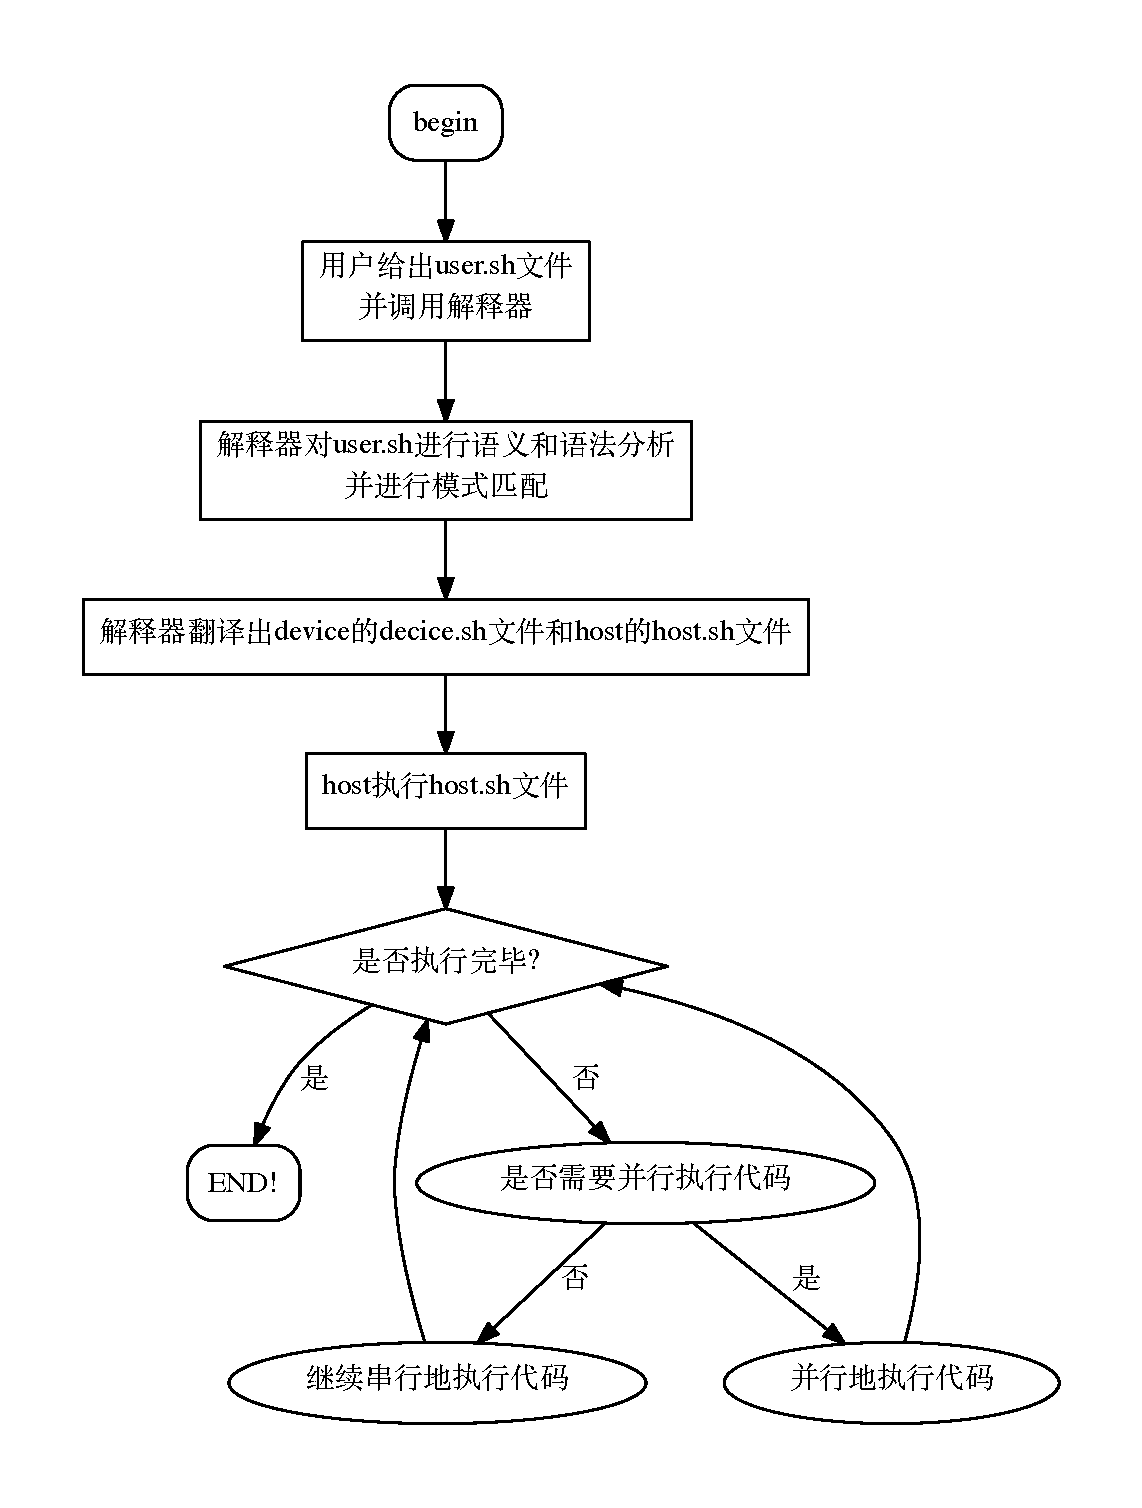
\includegraphics[width=1\textwidth]{pic/graph.pdf}
\caption{总体执行流程图}
\end{figure}

\begin{figure}[htbp]
\centering
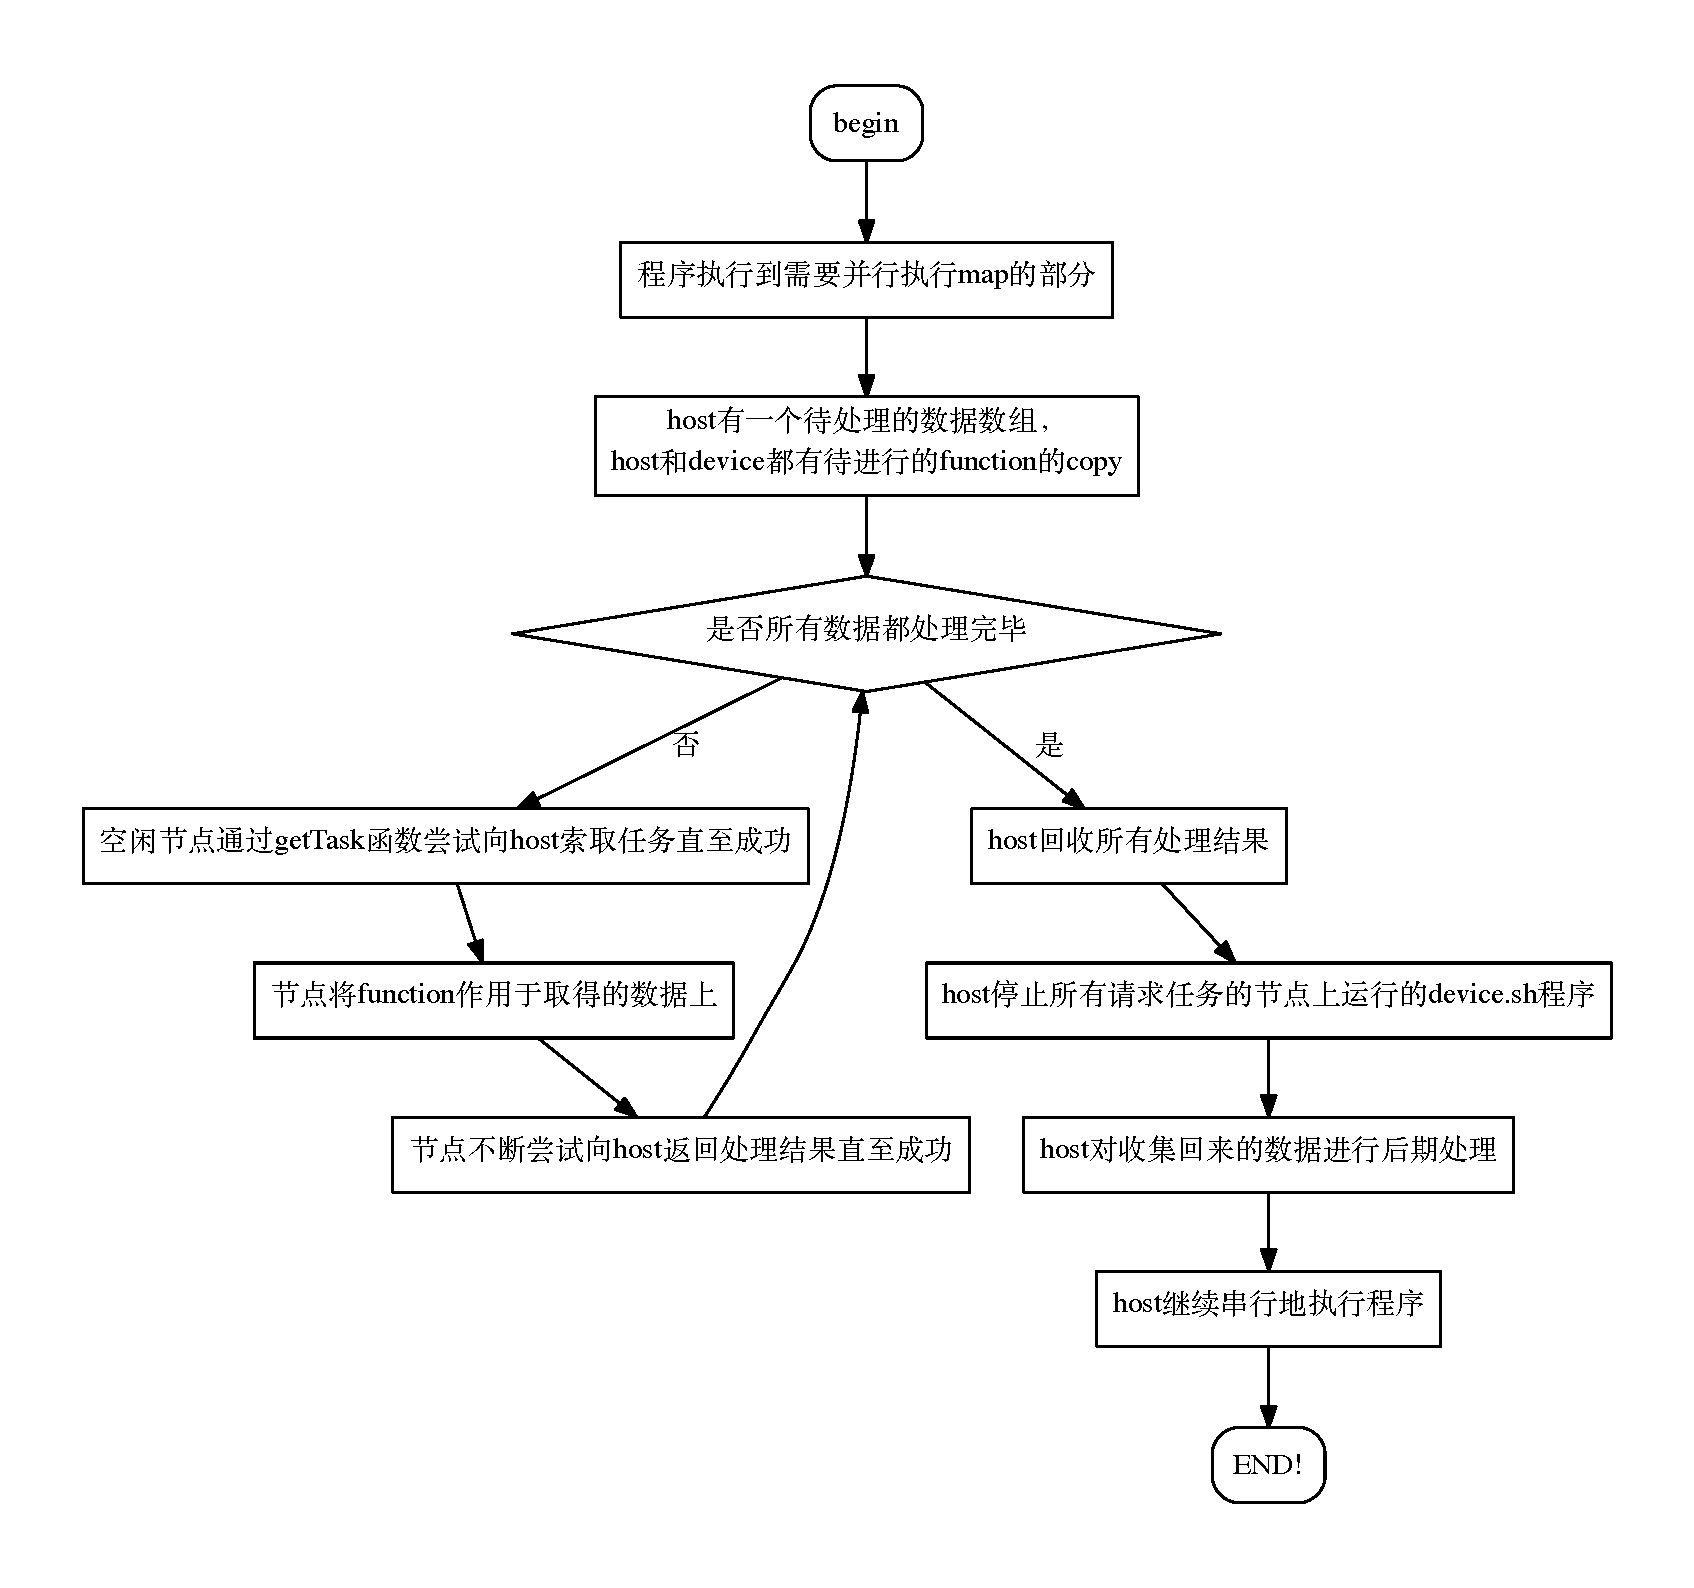
\includegraphics[width=1\textwidth]{pic/graph_map.pdf}
\caption{map执行流程图}
\end{figure}

\begin{figure}[htbp]
\centering
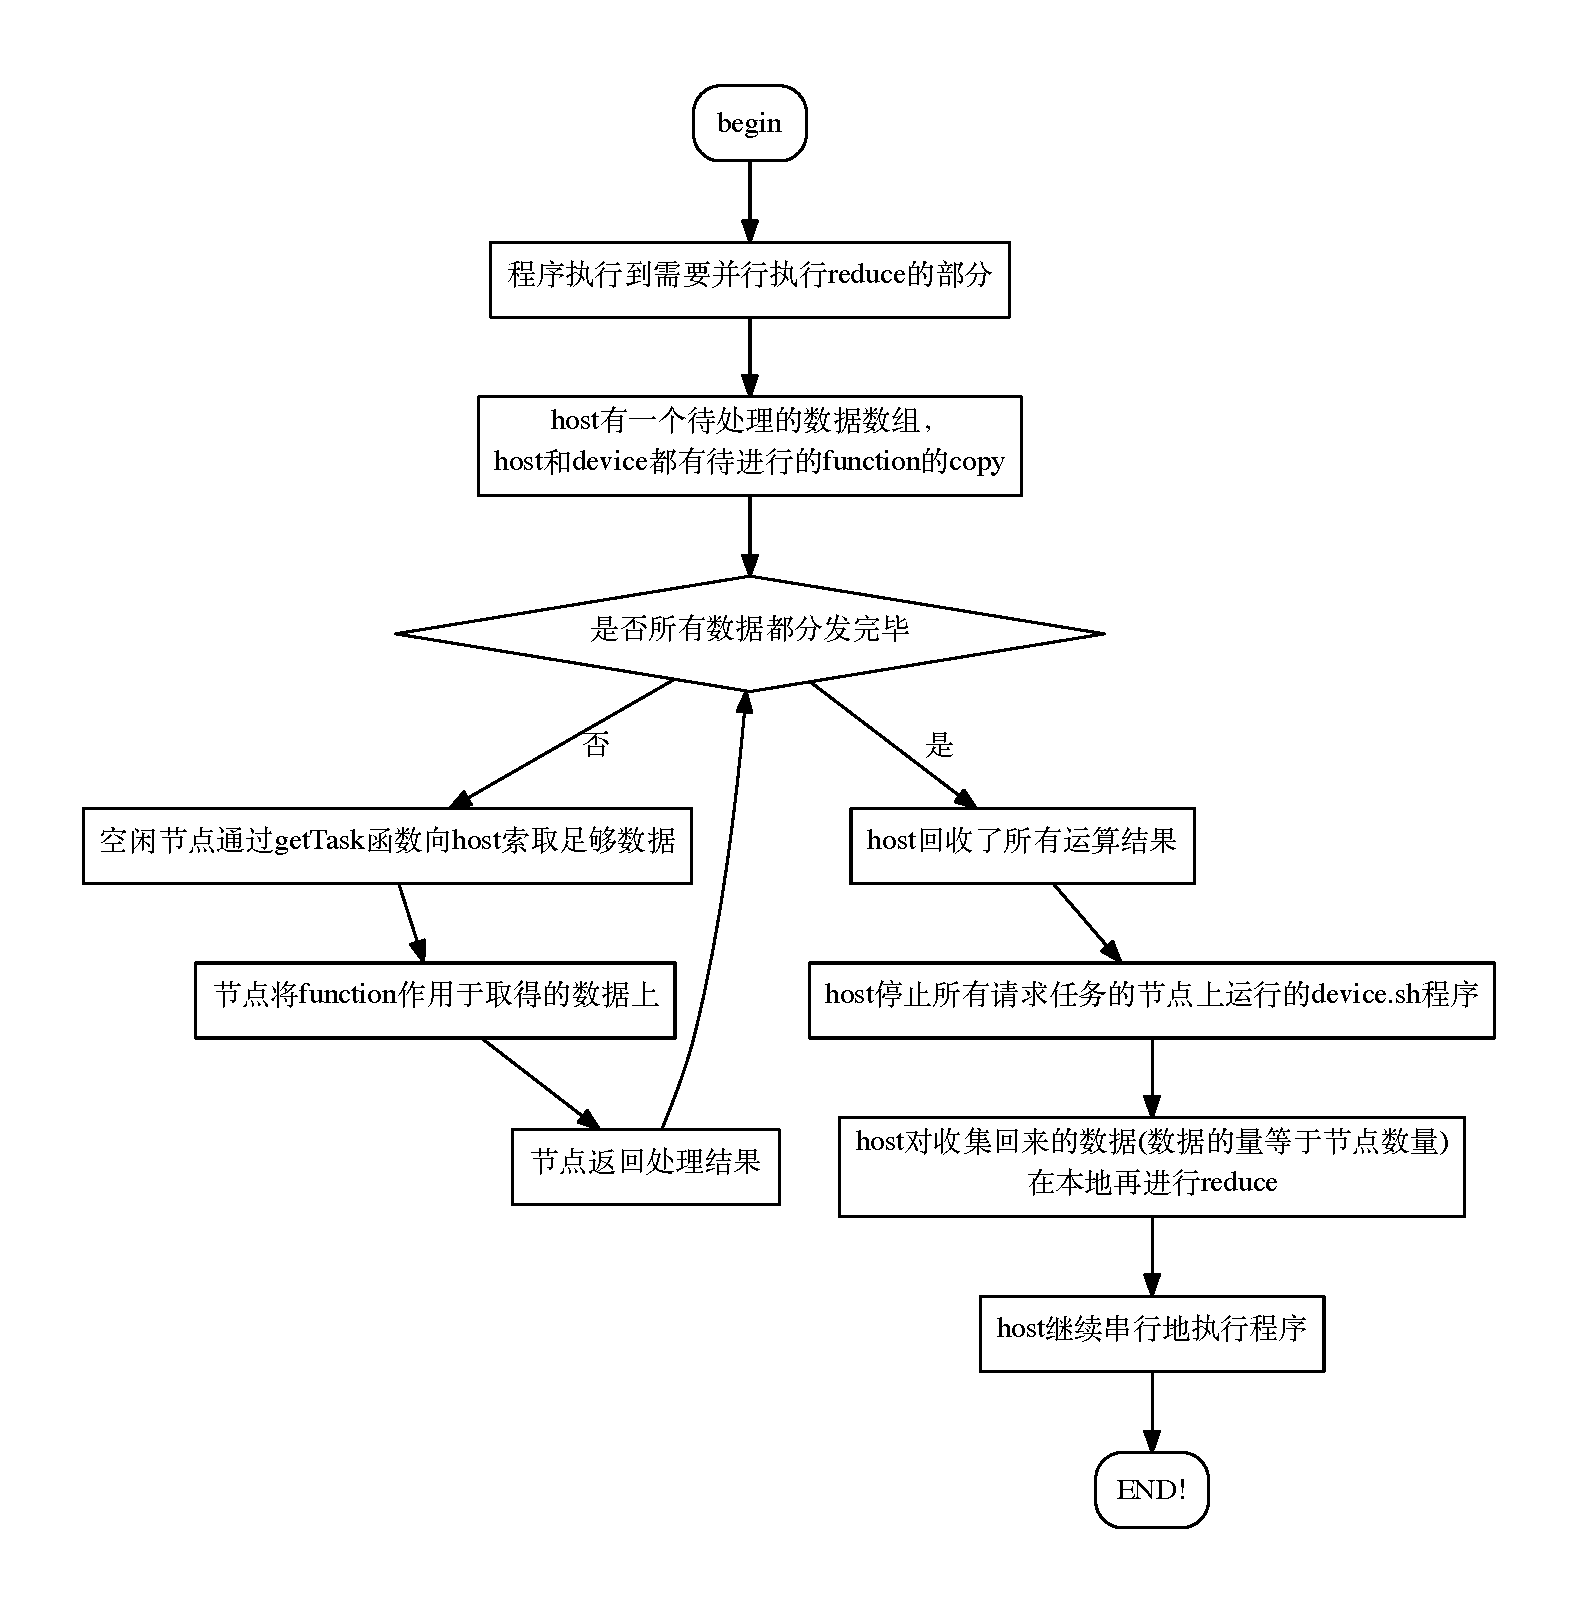
\includegraphics[width=1\textwidth]{pic/graph_reduce.pdf}
\caption{reduce执行流程图}
\end{figure}

\begin{figure}[htbp]
\centering
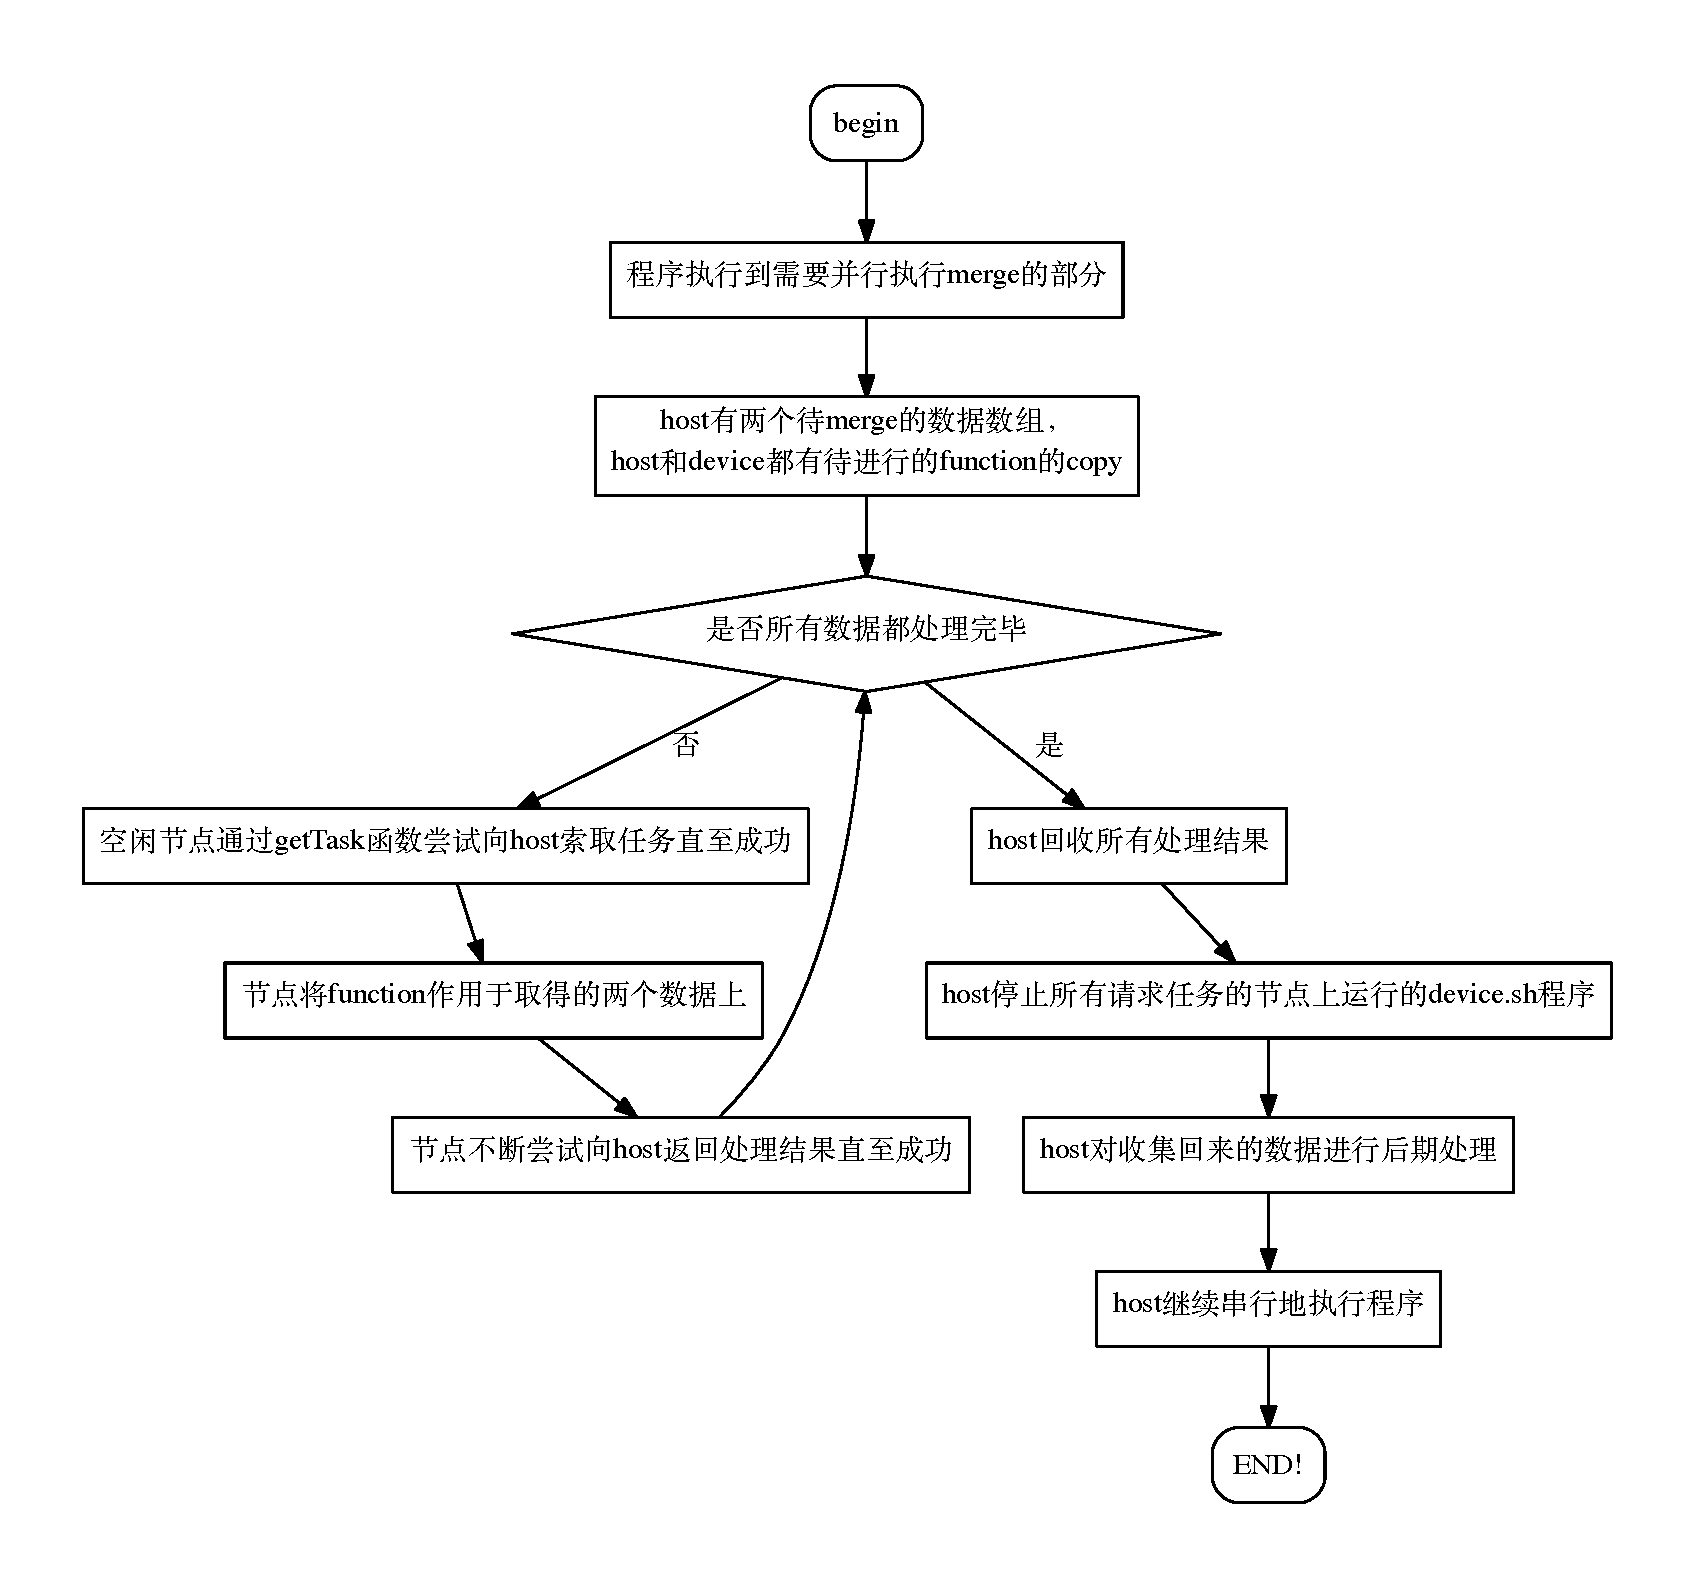
\includegraphics[width=1\textwidth]{pic/graph_merge.pdf}
\caption{merge执行流程图}
\end{figure}

\clearpage

\subsection{解释器的总体架构}

解释器的总体架构图如下:
\begin{figure}[htbp]
\centering
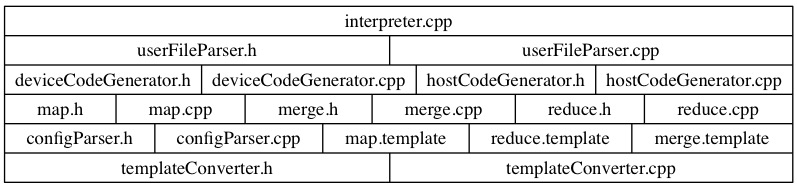
\includegraphics[width=1\textwidth]{pic/arch.jpg}
\caption{解释器的总体架构图}
\end{figure}

其中interpreter.cpp为顶层模块,为解释器的顶层架构代码.\n
第二层的userFileParser.h和userFileParser.cpp为user.sh的解析器,主要是对user.sh进行词法分析和语法分析提取出有关信息,便于第三层生成device和host代码.\n
第三层的deviceCodeGenerator.h与deviceCodeGenerator.cpp为device代码生成器. hostCodeGenerator.h与hostCodeGenerator.cpp为host代码生成器.它们使用第二层所得的信息分析并生成串行化部分代码,同时对并行部分进行类型判断并调用第四层的相应模块产生并行部分代码.\n
第四层为并行模块代码的生成器. map.h与map.cpp负责生成map部分的并行代码, merge.h与merge.cpp负责生成merge部分的并行代码, reduce.h与reduce.cpp负责生成reduce部分的并行代码.\n
第五层的configParser.h与configParser.cpp为template文件解析器.它会读入template文件并将其分块解析并缓存供第六层模块使用. map.template, reduce.template, merge.template为相应并行模块的template供configParser使用,他们是根据上文的3个函数并行化原理写成的模板文件,便于下层进行模式匹配.\n
第六层的templateConverter.h与templateConverter.cpp接受第五层的缓存信息,并结合上层传递下来的语法分析信息进行模式匹配,生成并行部分代码.


\section{并行计算框架的安装与用法}

\subsection{安装方法}
由于需要较多的源文件混合编译,我们采取使用GNU automake 和 autoconf套装进行自动化编译.用户需先安装>=1.11的automake以及>=2.13的autoconf.然后进入源文件夹执行./configure进行自动配置.然后再通过make,完成自动编译.最终通过make install将程序安装在/usr/bin中.若想清理编译的中间文件可执行make clean.

\subsection{配置device\_ip}
在运行并行程序之前,我们需要配置device的IP地址.配置十分简单,只需在源文件夹里创建device\_ip这一文件,首先填127.0.0.1代表localhost地址即host地址.接着再填入各个device的IP地址,注意各个地址之间需空一格.\n
示例 : 
\begin{lstlisting}
127.0.0.1 192.168.0.1 192.168.0.2
\end{lstlisting}

\subsection{user.sh的编写}
用户首先需编写user.sh,然后经解释器翻译成并行化代码再执行.所以user.sh的编写非常重要.\n
user.sh的语法格式和Inferno Shell及其相似.其中串行部分格式和Inferno Shell完全相同.并行部分格式如下:\n
\begin{lstlisting}
@parallel_begin
parallel code blocks.....
@parallel_end
\end{lstlisting}
其中parallel code blocks可以是map, reduce和merge.
一个完整的user.sh示例如下:

\lstinputlisting{code/user.sh}

\subsection{执行一个并行化程序}
只需进入Inferno终端,并进入工作目录/usr/inferno/parallel. 在此目录下编写user.sh.之后执行sh finish.sh即可完成对user.sh的翻译生成device和host代码. 

    \begin{figure}[htbp]
      \centering
      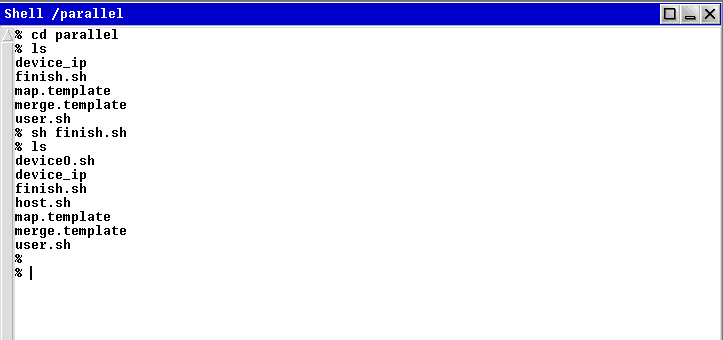
\includegraphics[width=\textwidth]{pic/inferno_interpreter.png}
      \caption{解释器解释user.sh生成device和host代码}
    \end{figure}

 之后再执行sh host.sh即可由host调度各个device进行并行化执行,得到结果.整个过程非常方便.

    \begin{figure}[htbp]
      \centering
      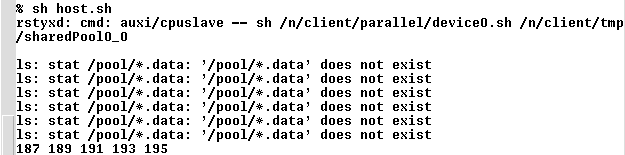
\includegraphics[width=\textwidth]{pic/sh_host.png}
      \caption{执行host.sh进行计算}
    \end{figure}

\section{成果与不足}

\subsection{向官方提交了2个bug与1个patch}

\subsubsection{arm架构下的编译bug}
发现arm架构下存在编译的bug.第一时间通知官方,并被标记位critical级别.不久在和官方的共同努力下成功修复此bug.

    \begin{figure}[htbp]
      \centering
      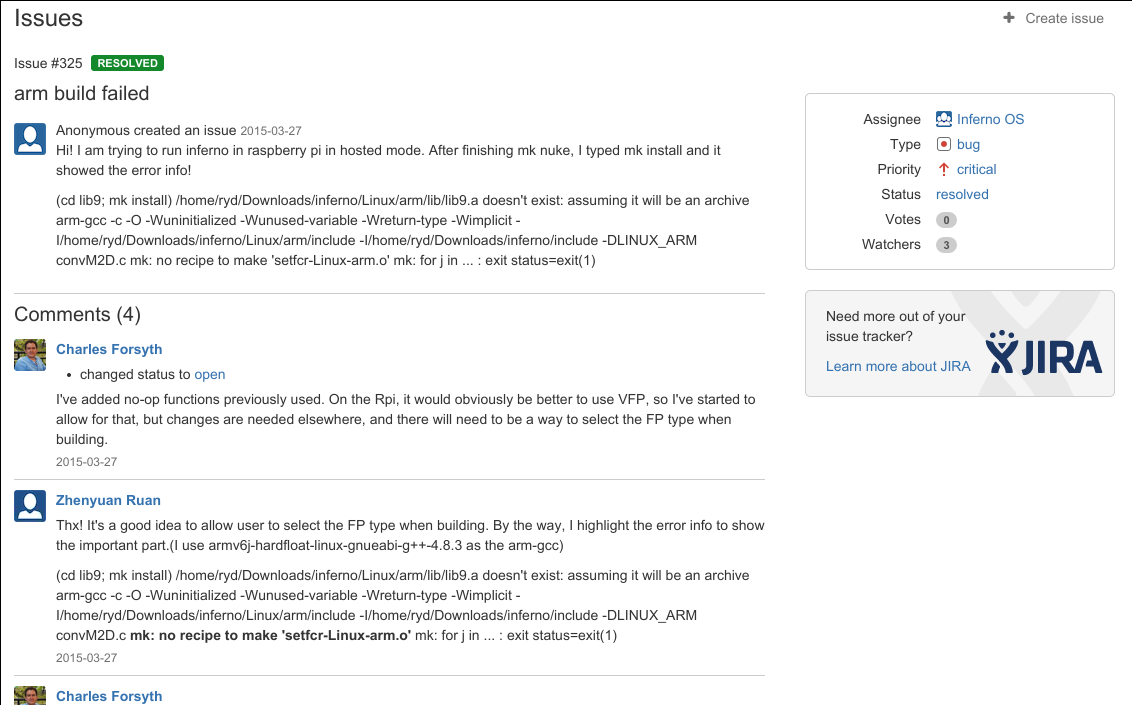
\includegraphics[width=1\textwidth]{pic/bug1.png}
      \caption{arm架构下的编译bug}
    \end{figure}

\subsubsection{arm架构下的网络接口bug}
发现了arm架构下网络接口存在问题,并第一时间通知官方.被官方标记未major级别.

    \begin{figure}[htbp]
      \centering
      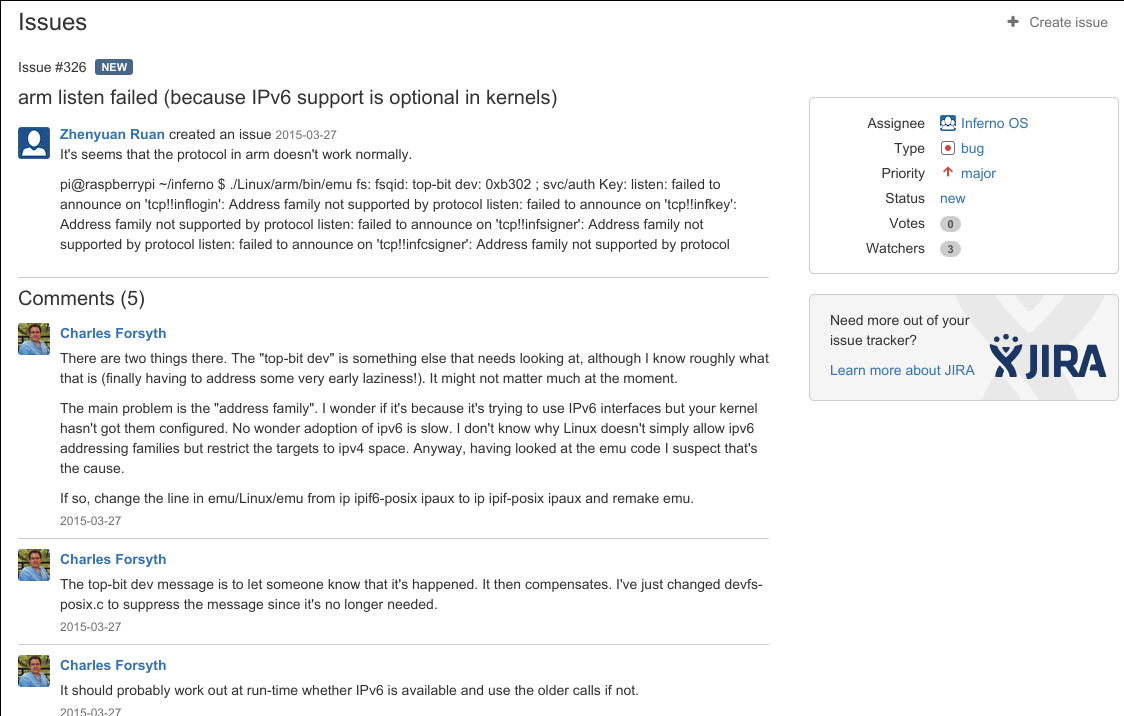
\includegraphics[width=1\textwidth]{pic/bug2.png}
      \caption{arm架构下的网络接口bug}
    \end{figure}

\subsubsection{有关x86编译问题的patch}
发现了x86下存在编译问题,第一时间修复并通知官方.官方告知不久之前他们也以修复,但还未来得及更新源码.

    \begin{figure}[htbp]
      \centering
      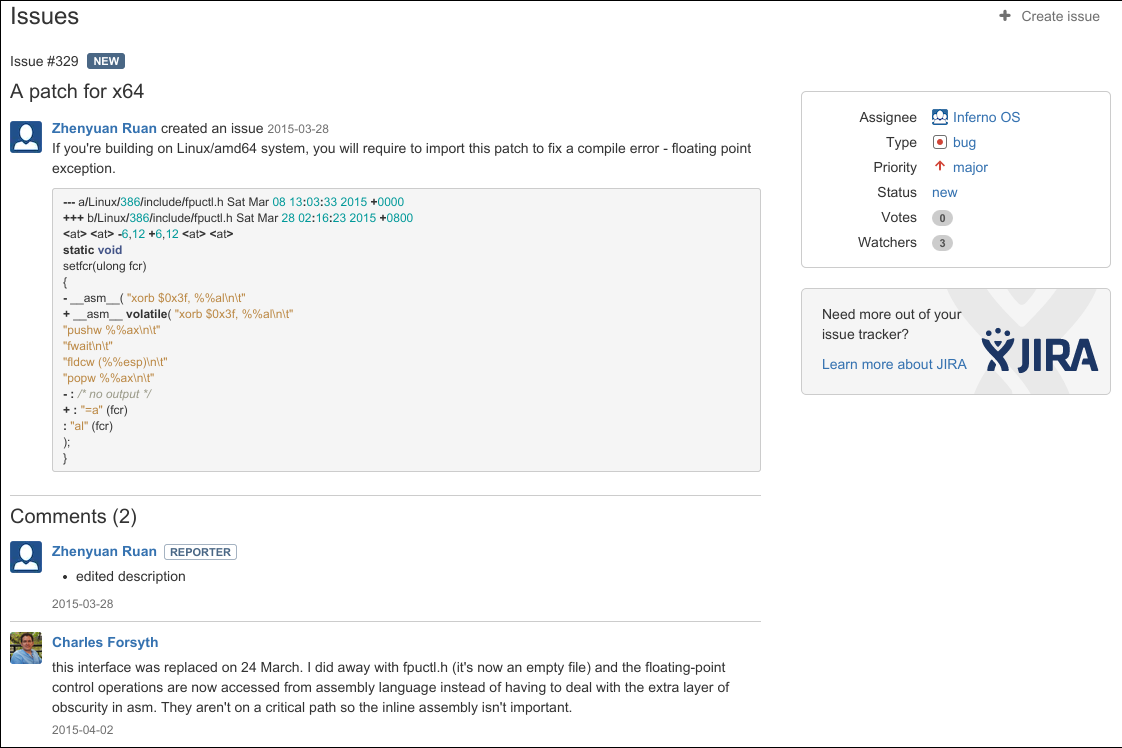
\includegraphics[width=1\textwidth]{pic/patch.png}
      \caption{有关x86编译问题的patch}
    \end{figure}

\subsection{日志功能方便调试}
 在程序的执行过程中,会在pool中产生log日志文件,包括host的日志host.log和每个device的日志,方便查看中间结果和调试程序。\n
    host.log的内容包括来提交计算结果的进程pid和提交结果之后的当前计算结果。如图:

    \begin{figure}[htbp]
      \centering
      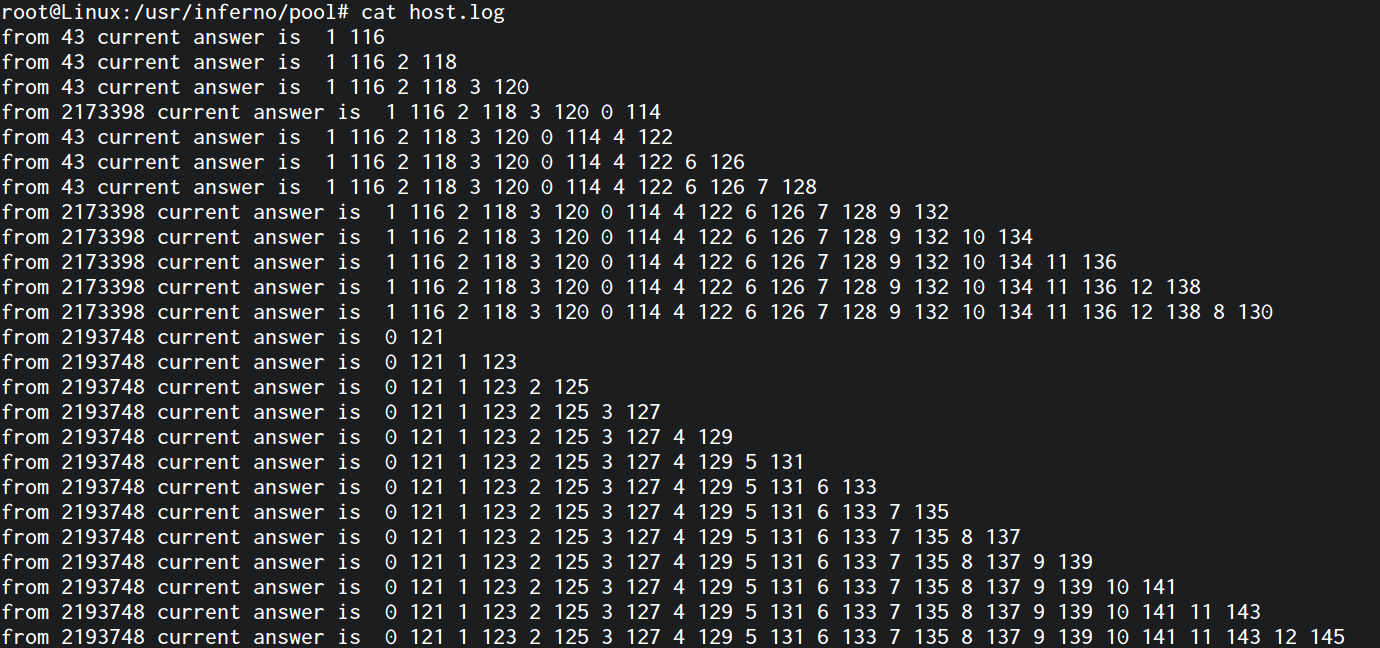
\includegraphics[width=1\textwidth]{pic/hostlog.png}
      \caption{host的日志}
    \end{figure}

    device的日志包括该节点获得的数据和将要提交给host的计算结果。如图:

\begin{figure}[htbp]
\centering
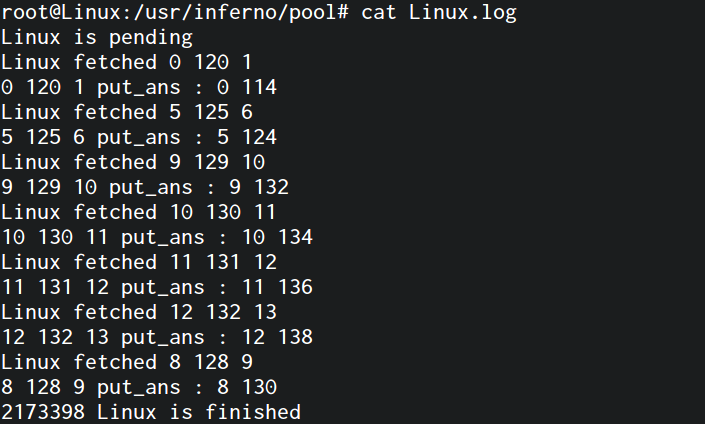
\includegraphics[width=1\textwidth]{pic/devicelog.png}
\caption{device的日志}
\end{figure}

\clearpage

\subsection{故障修复}
当macbook节点计算到编号为7的数据时,出现故障,对应黄色边框。\n
当yangzhi-GE70-0NC-GE70-0ND节点取得编号为11的数据时,出现故障,对应红色边框。\n
最后,当Linux节点处理完分配的任务后,重新计算之前出现故障的节点的数据,保证了最后结果的正确性。\n

\begin{figure}[h]
\centering
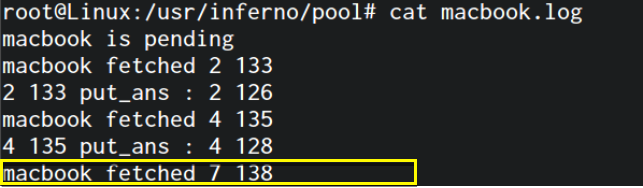
\includegraphics[width=1\textwidth]{pic/error2.png}
\caption{macbook节点取编号为7的数据时出现故障}
\end{figure}

\begin{figure}[h]
\centering
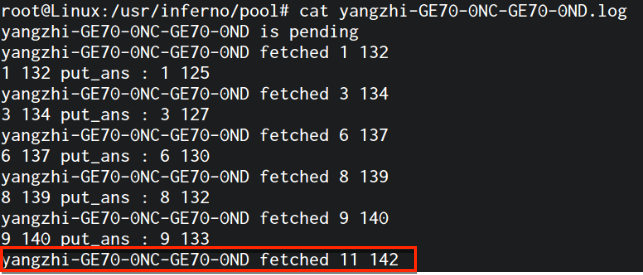
\includegraphics[width=1\textwidth]{pic/error3.png}
\caption{yangzhi节点取编号为11的数据时出现故障}
\end{figure}

\begin{figure}[h]
\centering
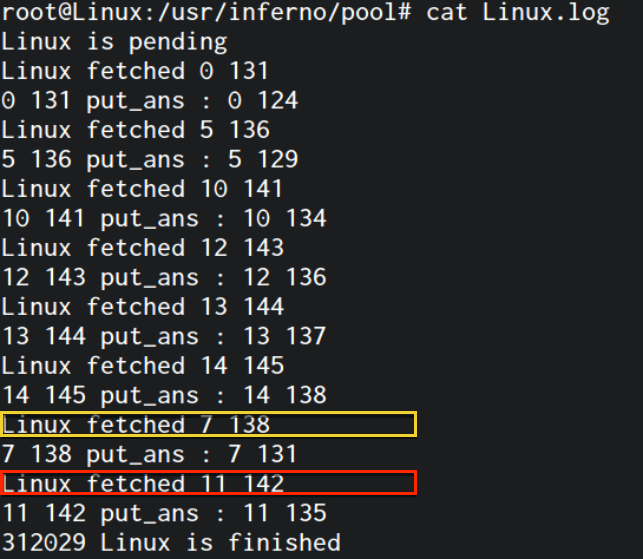
\includegraphics[width=1\textwidth]{pic/error1.png}
\caption{Linux节点在完成自身任务后重新计算因故障未被计算的数据}
\end{figure}

\subsection{跨平台性}
由于Linux, Unix以及Windows均支持hosted模式的Inferno,故此框架具有天然的跨软平台型.用户可以在不更改当前操作系统环境的条件下使用这套并行计算框架.这个使用者的部署(deploy)带来了极大的方便,只需本地安装Inferno并编译安装解释器即可使用. \n
同时由于Inferno自身支持x86, amd64, arm, spark, mips, powerPC等多种指令集体系结构,故此框架具有天然的跨硬平台型.\n
综上,此并行计算框架可以在各种软环境,硬平台下执行,给使用者带来了极大的方便.

\subsection{高度可扩展性与可配置性}
\begin{figure}[htbp]
\centering
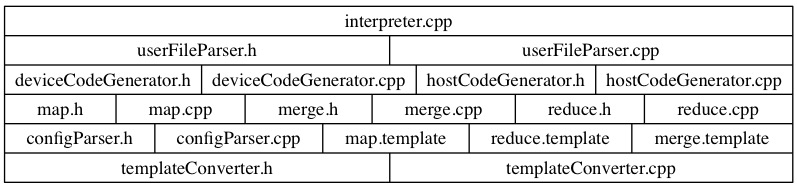
\includegraphics[width=1\textwidth]{pic/arch.jpg}
\caption{解释器的总体架构图}
\end{figure}
现在我们的并行计算框架仅有map, reduce与merge函数.然而介于解释器优良的架构,扩展其他函数变得非常的容易.由解释器的架构图可知,倘若我们想再往框架中添加fun1这个函数, 我们只需参照map.h与map.cpp的写法往第四层添加fun1.h和fun1.cpp.同时编写fun1对应的template,扩展第五层即可.整个扩展的过程非常简单,用户可以在不了解解释器底层工作原理的情况下轻松扩展解释器.\n
同时由于我们采用了template的机制,将解释规则和解释内容分隔开来.解释器中制订了一套规则,而具体解释成什么由template来定.解释器在读取user.sh进行语法分析之后,再读入template进行模式匹配完成翻译.若想优化翻译出的代码只需修改template即可,而解释器的内容可以一行不改.我们将解释器与template分离使其具有了高度的可配置型.

\subsection{benchmark}

\subsubsection{各个设备的配置}
我们使用了树莓派,以及组员四台电脑合计5台设备进行benchmark测试.其中五台设备的具体信息如下: 

\paragraph{树莓派}
型号 : Raspberry Pi 2\n
CPU : ARM Cortex-A7 @ 900MHz\n
RAM : LPDDR2 SDRAM 1GB\n
Disk : kingston 16GB SD Card.

\paragraph{刘旭彤的设备}
型号 : 2014款MacBook Air 13'低配\n
CPU : Intel Core i5-4260U @ 1.4 GHz \n
RAM : DDR3 4 GB 1600 MHz\n
Disk : Samsung SSD 128GB.

\paragraph{阮震元的设备}
型号 : 2013款MacBook Air 13'高配\n
CPU : Intel Core i5-4250U @ 1.3 GHz \n
RAM : DDR3 4 GB 1600 MHz\n
Disk : Samsung SSD 256GB.

\paragraph{解宇飞的设备}
型号 : Terrans Force x511 \n
CPU : Intel Core i7-4700MQ @ 2.40GHz\n
RAM : DDR3 16G 1600 MHz\n
Disk : 西部数据1TB 7200转\n

\paragraph{杨智的设备}
型号 : MSI G1790\n
CPU : Intel Core i7 3630QM @ 2.40GHz\n
RAM : DDR3 8G 1600 MHz\n
Disk : 日立 750GB 7200转\n

\subsubsection{benchmark内容}

我们采用检验给定表中素数个数来作为我们的压力测试(benchmark). 首先为了保证有一定计算压力,我们采用复杂度较高的试除法作为素数检验算法,而不是基于随机性的素数测试.试除法的检验数x是不是素数的过程如下:

\begin{enumerate}
\item 从2到根号x(取下整)枚举i,若枚举完毕则跳(3).
\item 检验x是否整除i,若整除则x是合数,否则返回(1).
\item x是素数.
\end{enumerate}

由于不个设备的性能,我们先在每个设备上运行串行版本的benchmark进行各个设备的性能基准测试.之后通过我们的并行框架将各个设备互联运行并行版本的benchmark. \n
我们选用了百余个大素数(十亿级别)掺杂着少量合数组成名为input的表.用试除法编写了名为isprime的subfn.再时编写了名为add的二元和函数.

\paragraph{串行版本的benchmark}
枚举input中的每个数字x,再用试除法判断x是不是素数,如果是使答案加1.最终输出答案.具体代码如下:
\lstinputlisting{serial.sh}

\paragraph{并行版本的benchmark}
首先通过map input isprime将input映射为只含0/1的表,素数被映射为1,合数被映射为0.最后通过reduce input add ans得到素数的总个数.具体代码如下: 
\lstinputlisting{parallel.sh}

\subsubsection{性能基准测试结果}
五台设备均运行串行版本的benchmark进行性能基准测试.如图所示,树莓派跑完benchmark的时间远超于其他设备,性能较差.刘旭彤的设备速度约比阮震元设备慢一倍.杨智的设备比阮震元的更快一些,解宇飞的设备速度最快.

\begin{figure*}[h*]
\centering
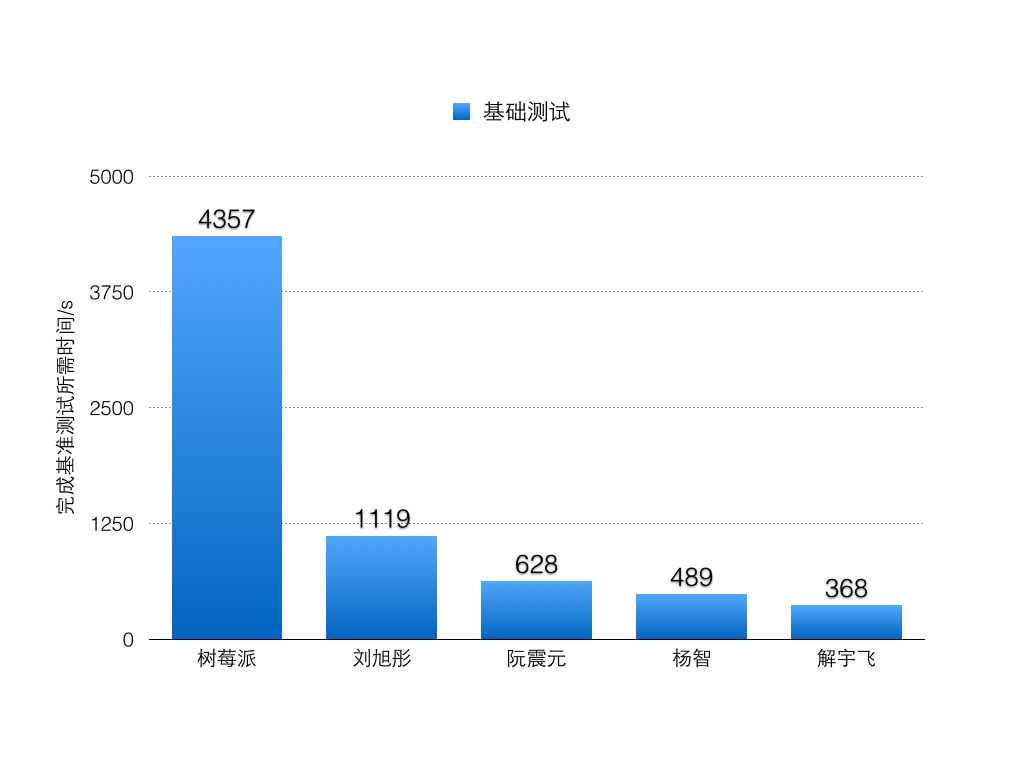
\includegraphics[width=\textwidth]{pic/graph001.jpg}
\caption{五台设备性能基准测试结果}
\end{figure*}

\subsubsection{使用并行计算框架进行并行benchmark测试}
所得结果如图所示.首先用树莓派使用并行计算框架的进行单节点测试(即虽然使用并行计算框架,但仅有树莓派这一个节点参与计算)所得时间为4493s,与树莓派运行串行代码相比略慢了一些.这是由并行计算框架中通讯以及同步耗时所带来的.\n
接着,树莓派加上刘旭彤设备进行双节点并行计算.仅需937s就跑完了整个benchmark,速度大幅提升.\n
加上阮震元的设备进行3节点并行计算仅需要307s.\n
加上解宇飞的设备进行4节点并行计算仅需要175s.\n
加上杨智的设备进行5节点并行计算仅需要110s.\n

\begin{figure*}[h*]
\centering
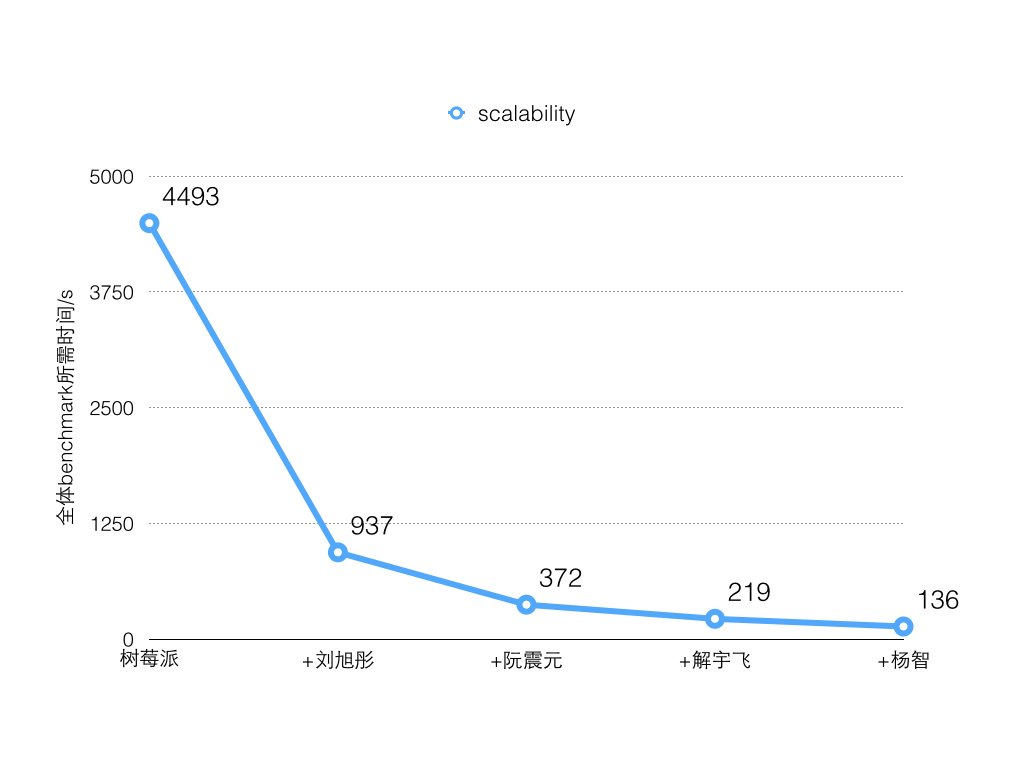
\includegraphics[width=\textwidth]{pic/graph003.jpg}
\caption{使用并行计算框架进行并行benchmark测试}
\end{figure*}

由以上结果我们可以计算出实际加速比.同时我们可以根据基准测试推算出加速比的理论值.将两者绘于一张图上进行比较.由图可知,我们的并行计算框架性能较好,实际加速比值接近理论加速比值.

\begin{figure*}[h*] 
\centering
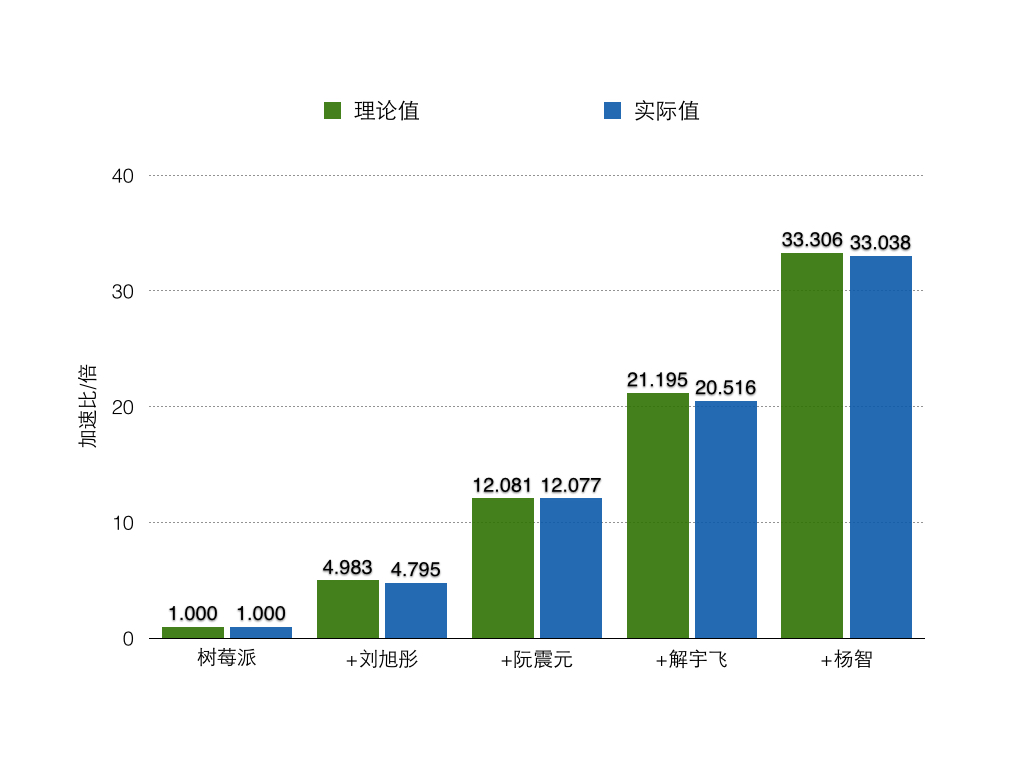
\includegraphics[width=\textwidth]{pic/graph004.png}
\caption{实测所得加速比与理论计算所得加速比(较单节点树莓派)}
\end{figure*}

\subsection{与其他并行计算框架的对比}

\subsubsection{异构性}

我们最终实现的并行计算框架异构性较好。\n
节点A运算完毕花了4357秒,节点B花了1119秒,节点C花了628秒,节点D花了489秒
,节点E花了368秒。但当这四个节点组成集群进行同一项测试时,只花了119秒就完成了。由此可见,运算较慢的节点A非但没有拖累整个集群的整体性能,反而提高了集群的运算速度。\n
另一方面,该并行计算框架不要求各节点的框架一致、不要求操作系统一致(Inferno可以安装在另一个操作系统上)、不要求硬件相似或者相同,只要节点能够运行Inferno,我们就能把它加入到集群中,提高集群的运算能力。\n
与MPI相比,我们在异构性这方面占了极大的优势。\n
一方面,使用MPI进行并行计算时,为了保证各个进程间的同步,有时候不得不调用名为MPI\_BARRIER的函数,通过这种方式阻止调用直到communicator中所有进程已经完成调用,实现同步。这种方式就有可能会导致运算速度慢的节点拖累其它节点的运算。\n
又如在MPI,以一种动态负载均衡算法为例,我们需要考虑cpu队列长度、cpu利用率、可用内存大小、上下文切换速度等因素来评价各节点负载状态,要决定如何收集系统当前负载的信息、是否进行任务迁移以及向何处迁移、如何进行迁移,一旦处理不好,就很容易出现硬件水平差的节点影响集群整体速度的情况。\n
另一方面,MPI还要求集群中的各个节点硬件相似或者相同,要求各节点是同一框架,异构性不好。

\subsubsection{部署简单}

\paragraph{我们的并行计算框架}

    下载之后只需./configure,/make,/make install三条命令即可安装。使用方法也非常方便,只需配置device\_ip,然后运行finish.sh即可生成并行化可执行代码。由于我们基于inferno分布式操作系统,所以我们生成的host和device代码只需存在host上即可,不需要把可执行的程序复制到每台机器上。非常易于使用.

\paragraph{CUDA}
为使用CUDA我们需要安装3个软件包,分别是:CUDA Driver,CUDA Toolkit,CUDA SDK。然后还要配置系统环境变量和编译环境,代码要经过专有编译器nvcc编译之后才可使用。使用起来较为麻烦.

\paragraph{MPI}
    首先要在每台机器上安装MPI套件,例如Intel MPI、OpenMPI等套装,有时在安装时要进行繁琐的编译参数配置,安装后要配置系统环境变量和编译环境,多台节点同时运行时要至少注册一个mpi账号,然后创建JOB目录,每台机器上必须有一个路径相同的目录,再将可执行文件复制到其它所有的机器上。使用起来非常麻烦.

\subsubsection{编程简单}
我们小组并行框架相对于主流并行框架拥有更强的易用性。下面我们就与主流并行框架:Open Mp,CUDA,OpenCL,MPI一一进行比较:

\paragraph{我们的并行计算框架}
我们小组的并行框架易用性是极强的,用户所需要做的只是按要求将函数和数组作为参数传入,在想要并行的部分之前加上@parallel\_begin,在结束的地方加上@parallel\_end,中间即为要并行的代码。举个例子,通过map操作将表array1中每个元素加1:

\begin{lstlisting}
subfn calculate {
    result = ${expr $1 1 +}
}
array1 = 120 121 122 123 124 125 126 127 128 129 130
@parallel_begin
map array1 calculate
@parallel_end
\end{lstlisting}
由此可见,即使是刚使用本框架的用户也可以极快上手。那些繁杂的并行化部分都是由解释器解决的,对于用户是透明的。

\paragraph{OpenMP}

OpenMP的编程还是相对简单的,我们以一个简单的for循环作为例子:
\begin{lstlisting}
#include <iostream>

using namespace std;

int main()
{
#pragma omp parallel for
    for (int i=0; i<10; i++) 
    {
        cout << i;
    } 
    return 0;
}
\end{lstlisting}
由上面的例子可以看出:要想将你的程序变为一个OpenMp的并行程序,只需加上一行代码\#pragma omp parallel for.简单的来说,就是将你想要并行化的代码加上OpenMp的并行标示\#pragma omp parallel就可以完成并行化(线程级别并行),具体的工作将交于编译器完成,也具有较强的易用性.

\paragraph{CUDA}
CUDA允许用户进行线程级的并行。用户需要先了解:CUDA的每一个线程都有其线程ID,线程的ID信息由变量threadIdx给出。threadIdx是CUDA C语言的内建变量,通常它用一个三维数组来表示。由此表示一维、二维和三维线程块(thread block)。这样,无论是数组、矩阵还是体积的计算,都可以使用CUDA进行运算。举两个NxN矩阵相加的CUDA实现为例子:

\begin{lstlisting}
// Kernel definition  
__global__ void MatAdd(float A[N][N], float B[N][N], float C[N][N]) {  
    int i = threadIdx.x;  
    int j = threadIdx.y;  
    C[i][j] = A[i][j] + B[i][j];  
}  
  
int main() {  
    ...  
    // Kernel invocation with one block of N * N * 1 threads  
    int numBlocks = 1;  
    dim3 threadsPerBlock(N, N);  
    MatAdd<<<numBlocks, threadsPerBlock>>>(A, B, C);  
    ...  
}  
\end{lstlisting}
可以看出用户需要先定义一种被称为内核函数(Kernel Functions)的C函数。内核函数使用关键字\_\_global\_\_来声明,运行该函数的CUDA线程数则通过<<<…>>>执行配置语法来设置。每一个执行内核函数的线程都由一个唯一的线程ID,这一ID可以通过在内核函数中访问threadIdx变量来得到。所以,用户要先定义内核函数再进行线程分配,这样就与我们小组并行框架的易用性有一定差距。

\paragraph{OpenCL}
OpenCL是通用的异构平台编程语言,为了兼顾不同设备,使用极为繁琐。将OpenCL编程步骤进行归纳,可得以下13步:

\begin{enumerate}
\item Discover and initialize the platforms.调用两次clGetPlatformIDs函数,第一次获取可用的平台数量,第二次获取一个可用的平台。
\item Discover and initialize the devices.调用两次clGetDeviceIDs函数,第一次获取可用的设备数量,第二次获取一个可用的设备。
\item Create a context(调用clCreateContext函数).上下文context可能会管理多个设备device。
\item Create a command queue(调用clCreateCommandQueue函数).一个设备device对应一个command queue。上下文conetxt将命令发送到设备对应的command queue,设备就可以执行命令队列里的命令。
\item Create device buffers(调用clCreateBuffer函数).Buffer中保存的是数据对象,就是设备执行程序需要的数据保存在其中。Buffer由上下文conetxt创建,这样上下文管理的多个设备就会共享Buffer中的数据。
\item Write host data to device buffers(调用clEnqueueWriteBuffer函数).
\item Create and compile the program.创建程序对象,程序对象就代表你的程序源文件或者二进制代码数据。
\item Create the kernel(调用clCreateKernel函数).根据你的程序对象,生成kernel对象,表示设备程序的入口。
\item Set the kernel arguments(调用clSetKernelArg函数).
\item Configure the work-item structure(设置worksize).配置work-item的组织形式(维数,group组成等).
\item Enqueue the kernel for execution(调用clEnqueueNDRangeKernel函数).将kernel对象,以及work-item参数放入命令队列中进行执行。
\item Read the output buffer back to the host(调用clEnqueueReadBuffer函数).
\item Release OpenCL resources(至此结束整个运行过程).
\end{enumerate}
由此可见:OpenCL中的核函数必须单列一个文件。OpenCL的编程一般步骤就是上面的13步,太长了,以至于要想做个向量加法都是那么困难。下面代码是一个例子,该函数是一个映射函数,但竟然要高达90余行的代码量,对于用户的易用性相当差。
\begin{lstlisting}
//核函数文件,HelloWorld_Kernel.cl
 __kernel void helloworld(__global double* in, __global double* out)
 {
     int num = get_global_id(0);
     out[num] = in[num] / 2.4 *(in[num]/6) ;
 }

//主函数文件,HelloWorld.cpp
//For clarity,error checking has been omitted.
#include <CL/cl.h>
#include "tool.h"
#include <string.h>
#include <stdio.h>
#include <stdlib.h>
#include <iostream>
#include <string>
#include <fstream>

using namespace std;

int main(int argc, char* argv[])
{
    cl_int    status;
    /**Step 1: Getting platforms and choose an available one(first).*/
    cl_platform_id platform;
    getPlatform(platform);

    /**Step 2:Query the platform and choose the first GPU device if has one.*/
    cl_device_id *devices=getCl_device_id(platform);

    /**Step 3: Create context.*/
    cl_context context = clCreateContext(NULL,1, devices,NULL,NULL,NULL);

    /**Step 4: Creating command queue associate with the context.*/
    cl_command_queue commandQueue = clCreateCommandQueue(context, devices[0], 0, NULL);

    /**Step 5: Create program object */
    const char *filename = "HelloWorld_Kernel.cl";
    string sourceStr;
    status = convertToString(filename, sourceStr);
    const char *source = sourceStr.c_str();
    size_t sourceSize[] = {strlen(source)};
    cl_program program = clCreateProgramWithSource(context, 1, &source, sourceSize, NULL);

    /**Step 6: Build program. */
    status=clBuildProgram(program, 1,devices,NULL,NULL,NULL);

    /**Step 7: Initial input,output for the host and create memory objects for the kernel*/
    const int NUM=512000;
    double* input = new double[NUM];

    for(int i=0;i<NUM;i++)
        input[i]=i;

    double* output = new double[NUM];

    cl_mem inputBuffer = clCreateBuffer(context, CL_MEM_READ_ONLY|CL_MEM_COPY_HOST_PTR, (NUM) * sizeof(double),(void *) input, NULL);

\end{lstlisting}

\paragraph{MPI}
MPI对于用户的要求也是很高的,MPI有几个很重要的概念rank, group, communicator, type, pack, spawn, window, 用户只有理解了这些概念才可能了解MPI框架的使用方法。而这几个概念是身份抽象的。比如说group这个概念,一台电脑可以属于多个group,group也可以随时随地的组合任意group,然后利用gourp内,和group间的communicator,可以很容易实现复杂科学计算的中间过程。例如奇数rank一个group,偶数另一个group,或者拓扑结构的group,这样可以解决很多复杂问题,另外MPI还有一个默认的全局的group,它就是comm world。\n
当然理解了这些概念也还是远远不够的,用户还需要掌握MPI的数据结构和许多编程技巧。比如一个简单的计算矩阵和的程序:

\begin{lstlisting}
#include "mpi.h"

#include <iostream>
#include <fstream>

int main(int argc, char* argv[])
{
	using namespace std;
	int rank;
	int size;
	MPI_Status Status;
	MPI_Init(&argc, &argv);
	MPI_Comm_rank(MPI_COMM_WORLD,&rank);
	MPI_Comm_size(MPI_COMM_WORLD,&size);

	const int MAXX=8;
	const int MAXY=3; 
	const int MAXPROCESSOR=64;
	float Data[MAXX][MAXX]; 
	int ArraySize[2];
	int i,j,k;

	if (rank == 0) 
	{
		ifstream in("input.txt"); 
		in>>ArraySize[0]>>ArraySize[1];
		for (i=1; i<=ArraySize[0]; i++ ) 
		{
			for (j=1; j<=ArraySize[1]; j++) 
			{
				in>>Data[i][j]; 
			}
		}
	}

	MPI_Bcast(ArraySize,2,MPI_INT,0,MPI_COMM_WORLD);
	int AverageLineNumber,HeavyProcessorNumber,MyLineNumber; 
	int CurrentLine,StartLine,SendSize; 
	float SendArray[MAXX*MAXY];

	AverageLineNumber=ArraySize[0] / size;
	HeavyProcessorNumber=ArraySize[0] % size; 
	if (rank < HeavyProcessorNumber) 
	{
		MyLineNumber=AverageLineNumber+1;
	}
	else
	{
		MyLineNumber=AverageLineNumber;
	}

	if (rank == 0)
	{
		CurrentLine=ArraySize[0]; 
		for (i=size-1; i >= 0; i--) 
		{
			SendSize=0; 

			if (i < HeavyProcessorNumber) 
				StartLine=CurrentLine-AverageLineNumber; 
			else 
				StartLine=CurrentLine-AverageLineNumber+1; 

			for (j=StartLine; j <= CurrentLine; j++) 
				for (k=1; k <= ArraySize[1]; k++) 
					SendArray[SendSize++]=Data[j][k]; 

			if (i != 0) 
				MPI_Send(SendArray,SendSize, 
						MPI_FLOAT,i,10,MPI_COMM_WORLD); 
			CurrentLine=StartLine-1;
		}
	}
	else
	{
		MPI_Recv(SendArray,MyLineNumber*ArraySize[1], 
				     MPI_FLOAT,0,10,MPI_COMM_WORLD,&Status); 
	}

	float *Sum=new(float); 
	*Sum=0; 
	for (i=0; i < MyLineNumber*ArraySize[1]; i++) 
		*Sum+=SendArray[i]; 
	float AllSum[MAXPROCESSOR];
	std::cout << "rank:" << rank << " cal sum is " << *Sum << std::endl;
	MPI_Gather(Sum,1,MPI_FLOAT,AllSum,1,MPI_FLOAT,0,MPI_COMM_WORLD); 

	if (rank == 0)
	{
		*Sum=0; 
		for (i=0; i < size; i++) 
			*Sum+=AllSum[i];
		cout<<"The Sum of the Array is:"<<*Sum<<endl; 
	}
	
	MPI_Finalize(); 
	return 0;
} 
\end{lstlisting}
由此可见,MPI对于用户的要求很高。完全无法想象一个刚接触MPI的用户如何能写出MPI框架下并行的代码。MPI的易用性也因此大打折扣,和我们小组相比有很大的差距。

\subsubsection{支持故障恢复}
    MPI标准并没有提供容错的策略,在MPI-1中任务和主机都是静态的,应用程序需以一个任务组的方式运行,当任务组中的一个任务或计算资源失败以后,整个应用程序都将失败,这是MPI标准对错误的处理方式。由于MPI标准中目前还缺乏关于容错的接口与操作的明确定义,众多的MPI版本需要在软件实现时解决容错问题。目前有一些MPI版本可以实现检查点设置/回卷恢复的功能。\n
    基于分布式系统和数据冗余的方法,我们的并行框架可以做到任何device出现故障不影响程序的执行和结果的正确性,当host出现故障才会中断程序执行。

\begin{table}[h]
  \footnotesize
  \large
  \caption{summary}
  \begin{tabular}{|c|c|c|c|c|c|} 
    \hline
    ~ & 我们的框架 & CUDA & MPI & OpenCL & OpenMP \\\hline
    异构性 & good & good & bad & good & $\backslash$ \\\hline
    部署难度 & easy & normal & normal & normal & easy \\\hline
    编程难度 & easy & normal & hard & crazy & easy \\\hline
    故障恢复 & support & $\backslash$ & unsupport & $\backslash$ & $\backslash$ \\\hline
    \end{tabular}
\end{table}

\subsection{不足点}
\begin{itemize}
\item 无法加速时间复杂度小于$O(n^2)$的算法(或者函数),例如对n个数据求和。具体的原因是host节点将数据分发出去,由于各个节点计算速度不同,收回结果的函数必定是乱序的。我们小组对于乱序的结果必须要进行排序,也就是说要根据pid为关键字进行排序。由于Inferno系统的自身因素,排序算法只能达到$O(n^2)$。所以本身时间复杂度小于$O(n^2)$的无法进行加速.
\item 由于我们小组使用的是Inferno的内嵌语言,类似于JVM,是对程序是进行逐行解释运行的。这导致我们小组设计的框架速度受限。
\item 我们小组使用了host-device平台模型。这就说明host一旦宕机整个系统就会崩溃,无法再进行故障修复。但是,经过我们查阅了大量的资料发现:大量并行框架也是采用此模型,如CUDA、OpenCL。可以预见,这两种模型也会出现类似的问题。当然,对于MPI,由于使用了广播与点对点结合的通信方式,任务发起者一旦宕机,同样也无法恢复。综上,这点不足也正是业界亟待解决的难题。
\end{itemize}

\subsection{完成过程中遇到的困难}
\begin{itemize}
\item 起初在64位Linux上编译inferno源代码无法通过,还有在移植到arm平台上遇到bug,通过查阅资料,并和inferno官方人员交流,最终成功将其移植到64位的平台和Raspberry Pi上。
\item 由于inferno系统普及程度不高,导致可以参考的资料非常匮乏,几乎只有官方网站上仅有的一点资料,给深入地学习带来困难,需要不断自己摸索尝试。
\item inferno系统提供的shell脚本语言功能有限,给代码编写造成困难,比如inferno的shell语言没有数组,导致map和merge函数并行部分结束之后必须进行表排序,降低了执行效率。 
\item inferno系统偶尔出现命令执行结果不稳定的bug,导致3个并行函数中作为计算完成标志的finish文件不能删除,然而不影响计算结果的正确性,令人比较困惑。还会出现输入运行程序命令后,一段时间没有反应,输入若干次回车之后才有反应的情况。
\item 起初在三台以上节点上运行时,file2chan分发任务不正确,经过查阅资料、阅读源代码,并做了大量实验之后,找到了解决方法,可以正确运行在多台机器上。
\item 由于inferno系统不是很完善,代码执行出错后提供的错误信息很少,并且调试工具不完善,导致程序调试困难,只能通过检查代码和输出变量的方式,降低了开发的效率。
\end{itemize}


\section{致谢}
本项目是在邢凯老师的悉心指导下完成的。\n
首先十分感谢邢凯老师,给与我们极大的关心与帮助,为我们提供许多问题解决的方案。其次十分感谢Inferno原作者Charles Forsyth,感谢他与我们进行了有益的探讨,一同解决了Inferno在amd64下编译的问题以及在arm环境下Inferno编译和网络接口问题。感谢Pete Elmore的博文为我们带来灵感。感谢安虹老师为我们提供研究场所,让我们专心研究课题。感谢张智帅学长为我们提供树莓派以及嵌入式开发板。感谢余家辉学长与我们进行了众多有益的探讨。最后感谢队友之间的集思广益、通力合作,以最高效的方式解决了各种棘手的问题。
 

        \begin{thebibliography}{99}
        \bibitem{1} https://en.wikipedia.org/wiki/Inferno\_(operating\_system), Inferno wikipedia
        \bibitem{1} https://en.wikipedia.org/wiki/Plan\_9\_from\_Bell\_Labs, Plan 9 wikipedia
        \bibitem{1} http://www.vitanuova.com/inferno/info/Inferno\_overview.pdf, Inferno Overview
        \bibitem{1} http://www.vitanuova.com/inferno/info/Inferno\_info.pdf, Inferno Information Sheet
        \bibitem{1} http://www.vitanuova.com/inferno/papers/bltj.html, The Inferno Operating System
        \bibitem{1} http://www.vitanuova.com/inferno/papers/styx.html, The Styx Architecture for Distributed Systems
        \bibitem{1} http://www.vitanuova.com/inferno/man/index.html, Inferno Manual Pages
        \bibitem{1} The Inferno Shell, Roger Peppé 
        \bibitem{1} http://debu.gs/entries/inferno-part-0-namespaces, Inferno Part 0: Namespaces
        \bibitem{2} http://debu.gs/entries/inferno-part-1-shell, Inferno Part 1: Shell
        \bibitem{2} The comparisons of opencl and openmp computing paradigm, SL Chu, CC Hsiao
        \bibitem{1} 不同层次MPI并行程序容错的比较, 赵毅,曹宗雁,朱鹏,迟学斌, 《e-Science技术》2011年11月第2卷第6期
        \bibitem{1} Fault Tolerant MPI, Graham E. Fagg, Jack J. Dongarra, FT-MPI, Supporting Dynamic Applications in a Dynamic World
        \bibitem{1} Fault-Tolerant Metacomputing and Generic Name Services: A Case Study, David Dewolfs, Jan Broeckhove, Vaidy Sunderam, Graham E. Fagg, FT-MPI, 
        \bibitem{1} A framework for parallel distributed computing, V. S. Sunderam,PVM
        \bibitem{1} PerfExplorer: A Performance Data Mining Framework For Large-Scale Parallel Computing, Kevin A. Huck, Allen D. Malony
        \bibitem{3} Open MPI: Goals, Concept, and Design of a Next Generation MPI Implementation, Edgar Gabriel, Graham E. Fagg, George Bosilca, Thara Angskun, Jack J. Dongarra, Jeffrey M. Squyres, Vishal Sahay, Prabhanjan Kambadur, Brian Barrett, Andrew Lumsdaine, Ralph H. Castain, David J. Daniel, Richard L. Graham, Timothy S. Woodall
        \bibitem{4} Teaching Parallel \& Distributed Computing with MPI, Joel C. Adams, Richard A. Brown, Elizabeth Shoop
        \bibitem{5} A parallel sampling based clustering, Aditya AV Sastry, Kalyan Netti
        \bibitem{6} GPGPU Computing Bogdan Oancea, Tudorel Andrei, Raluca Mariana Dragoescu
        \bibitem{7} Research on Multi-Core PC Parallel Computation Based on OpenMP Lan Xiaowen  
        \bibitem{8} Design of OpenCL framework for embedded multi-core processors, Jung-Hyun Hong, Young-Ho Ahn, Byung-Jin Kim, Ki-Seok Chung
        \end{thebibliography}
      \end{document}

\end{document}
 
%%% Local Variables:
%%% mode: latex
%%% TeX-host: t
%%% TeX-master: t
%%% End:  